\documentclass[12pt, a4paper,twoside]{tesi_upf}

\usepackage{pgfgantt}
\usepackage{tikz}
\usepackage{eurosym}
\usepackage{float}
\usepackage{pdfpages}

\usetikzlibrary{shapes.geometric, arrows}

\tikzstyle{startstop} = [rectangle, rounded corners, minimum width=3cm, minimum height=1cm,text centered, draw=black, fill=red!30]

\tikzstyle{io} = [trapezium, trapezium left angle=70, trapezium right angle=110, minimum width=3cm, minimum height=1cm, text centered, draw=black, fill=blue!30]

\tikzstyle{process} = [rectangle, minimum width=3cm, minimum height=1cm, text centered, text width=3cm, draw=black, fill=orange!30]

\tikzstyle{decision} = [diamond, minimum width=3cm, minimum height=1cm, text centered, draw=black, fill=green!30]

\tikzstyle{arrow} = [thick,->,>=stealth]

%CODIFICACIÓ
%\usepackage[latin1]{inputenc}
\usepackage[utf8]{inputenc}
%\usepackage[T1]{fontenc}
%\usepackage{lmodern}


%IDIOMES
\usepackage[catalan,english]{babel}

%NOMÉS PER A OBTENIR INDICACIÓ DEL MARC EN MIDA A4
%\usepackage[cam,a4,center,frame]{crop}

%PER A INCLOURE GRÀFICS I EL LOGO DE LA UPF
%\usepackage{graphicx}

\usepackage{caption}
\usepackage{subcaption}

\usepackage{graphicx}

\usepackage{caption}
\usepackage{acronym}
\usepackage{multirow}
%FONTS TIMES O GARAMOND, 
\usepackage{times}
%\usepackage{garamond}
\usepackage{url}

\usepackage{pdfpages}
%SENSE HEADINGS: NO MODIFICAR
\pagestyle{plain}

%PER A L'ÍNDEX DE MATÈRIES
\usepackage{makeidx}
\makeindex

%ESTIL DE BIBLIOGRAFIA
\bibliographystyle{apalike}


%AQUEST DOCUMENT ÉS EN CATALÀ
\selectlanguage{english}

%EN COMPTES DE ÍNDEX, LA TAULA DE CONTINGUTS ES TITULA SUMARI
\addto\captionscatalan
  {\renewcommand{\contentsname}{\Large \sffamily Sumari}}

% ~~~~~~~~~~~~~~~~~~~~~~~~~~
% CUSTOM PACKAGES
% ~~~~~~~~~~~~~~~~~~~~~~~~~~
%\usepackage{hyperref}
\usepackage[hidelinks]{hyperref}
\usepackage{titlesec}
\setcounter{secnumdepth}{4}
\usepackage{pdfpages}

%AFEGIU EN AQUESTA PART LES VOSTRES DADES
\title{A bottom up sensor testbed}
\author{Sergio Almendros Díaz}
\thyear{2014}
\department{Departament de Tecnologies de la Informacio i les Comunicacions (DTIC)}
\supervisor{Jaume Barcelo and Davide Scaini}


\begin{document}

\pdfstringdefDisableCommands{%
\let\MakeUppercase\relax
}

\frontmatter

\maketitle

\cleardoublepage


%%%%%% Dedicatòria; si no es vol posar, comenteu fins a final de dedicatòria

\noindent Dedicated to my parents and sister for supporting and helping me at any moment, and all my colleagues who have been with me all these years.

\cleardoublepage


%%%%%% Final de dedicatòria


%%%%%% Agraïments; si no es vol posar, comenteu fins a final de agraïments
\noindent {\Large \sffamily Acknowledgments}
\\

	First and foremost I want to thank my supervisor Jaume Barcelo for guiding and helping me throughout the whole project. I would also like to thank Davide Scaini for proposing the project and help me with the final report, to Manuel Palacin for helping me with technical issues and to Albert Domingo for his constructive criticism that made me progress.

	I also want to thank the other fellows: Ferran Selva, Pedro Vilchez, and Ivan Fernandez for helping in any way they could. 
	I would like to thank Alejandro Juez, Daniel Valderas, Jacob Uribe, Carles Xavier Vilás, and Aitor Rodriguez, whose experience and knowledge have helped me finish this project. 
	I also want to thank my family for supporting me since I started this project.

	Finally, my sincere gratitude to all my friends who have accompanied me in all the endless hours in the library.

\cleardoublepage

%%%%%% Final dels agraïments

%ABSTRACT EN DOS IDIOMES. COM A MÍNIM CATALÀ. SI L'ALTRE ÉS EN CASTELLA CANVIEU EL QUE POSA ABSTRACT
\selectlanguage{english}
\section*{\Large \sffamily Abstract}
 
  This project aims at creating a sensor testbed that can be continued and supported by a community. 
  The sensors gather environmental data and are connected to a community network. It gives the community a trace to improve their environmental conscience, giving them the necessary information to know the state of their surroundings and act accordingly.
  This way anybody can act consequently if the sensors detect harmful situations, for example, not going to a park where the gas sensor detects bad air quality.
  
  The sensor data is uploaded to a data broker developed by the University, which makes the data available to third-party applications. 
  A mobile application that connects to the data broker has been programmed. 
  This application offers an intuitive and meaningful visualization of sensor's data, tailoring its presentation to people without specific scientific knowledge.


\selectlanguage{catalan}
%\vspace*{\fill}
\section*{\Large \sffamily  Resum}

	Aquest projecte té com a objectiu desplegar un banc de proves de sensors que pot ser continuat i suportat amb el suport d'una comunitat.
	Els sensors recullen dades medioambientals i están connectats a una xarxa de la comunitat. Li dóna a la comunitat un camir per millorar la seva consciència ambiental, donant-los la informació necessària per conèixer l'estat del seu entorn i actuar en conseqüència. 
	
	D'aquesta manera tothom pot actuar en conseqüència si els sensors detecten situacions perilloses, per exemple, no anar a un parc en el qual el sensor de gas detecta mala qualitat de l'aire.
	Les dades del sensors s'emmagatzema en un data broker desenvolupat per la universitat, el que fa que les dades estiguin disponibles per a aplicacions de tercers.
	
	Una aplicació mòbil que es connecta al data broker ha estat programada. 
	Aquesta aplicació ofereix una visualització de les dades de sensors intuïtiva i significativa, adaptant la presentació de les dades per a persones que no tenen coneixements científics específics.

%\vspace*{\fill}

\selectlanguage{english}
\cleardoublepage
%FIN DE ABSTRACTE

%PREFACI OPCIONAL. SI NO ES VOL, COMENTEU FINS EL FINAL DE PREFACI
%{\bf Prefaci}
%
%\cleardoublepage
%FINAL DE PREFACI


%TAULA DE CONTINGUTS: OBLIGATÒRIA
\selectlanguage{english}
\tableofcontents

%INDEX DE FIGURES; NOMÉS ES POSA SI HI HA FIGURES
\listoffigures
%Fa que aparegui al sumari
\addcontentsline{toc}{chapter}{List of figures}

%INDEX DE TAULES; NOMÉS ES POSA SI HI HA TAULES
\listoftables
%Fa que aparegui al sumari
\addcontentsline{toc}{chapter}{List of tables}


%COMENÇA EL TEXT
\mainmatter
\chapter{Introduction}
\label{Chapter1}
	
	Sensor networks started as a mechanism of defense developed by the United States Navy during the Cold War. With acoustic sensors they searched for Soviet submarines. This research continued at Universities, trying to make the sensors smaller, and with the possibility of real-time data adquisition and processing \cite{chong2003sensor}.
	
	A sensor network is composed of nodes, and nodes are composed of computers and sensors. The function of these computers are: understand the data returned by the sensors, encapsulate it, and send it to the outside.
	
	A node is typically powered by batteries and because it would be unpractical to change batteries at short intervals, the node must require low power to perform all its functions. For this reason, these computers must be equipped with the minimum amount of hardware to perform these functions.
	To speed the deployment of the network, the most common are ad-hoc wireless sensor networks, which means that nodes will send data from node to node until it finds the target node. The goal is to keep all information collected by all sensors and work with it.
	In this case, an existing community network has been used, so the communication stage is not part of this project.
	
  The development of this project has been divided into three phases: collect data from environmental sensors, display it to end users in an intuitive way, and make a real testbed to demonstrate its performance.
  
  As a sensor node an Arduino\cite{arduino} YUN has been used, which allows to obtain easily analog reads from a sensor. With a Power over Ethernet module, it can be attached to Guifi\footnote{\url{http://guifi.net/}} nodes and send the sensor data to a sensor platform, e.g. Opencities \cite{opencities}.

  The Bottom-up\footnote{\url{http://bubforeurope.net}} pattern has been used to build the sensor testbed, where the end users, in this case, Guifi users, are the ones who has to assemble the sensor nodes and connect them to their Guifi nodes to create the sensor network. With the Bottom-up model, the data is provided and used by the users.

  In this project an Android application has been developed to visualize the sensor data and make it accessible to the final users.
  A sensor testbed has been deployed to gather sensor data, and test the technologies used and developed.
  
  This project is an attempt to understand the structure, the technological challenges and operations of sensor networks and how they can help us to take conscience about our environment.

  The thesis is structured as follows: the current state of sensor networks (Chapter \ref{Chapter2}), which technologies had been used (Chapter \ref{Chapter3}), and how the project has been developed (Chapter \ref{Chapter4}). 
  In chapter \ref{Chapter5} the testbed deployment is illustrated and some resulting data are shown.
  Finally, the conclusions (Chapter \ref{Chapter6}) and future work (Chapter \ref{Chapter7}).
  
\chapter{State of the Art}
\label{Chapter2}
  
  \section{Introduction}

    Currently the sensors are small enough to put several into a shield of the size of a credit card.
    
    Smart cities are the next step. A city capable of having real-time information, not only about the environment, but also from the number of cars that pass on a road, to the amount of rain water in a day. This kind of information could help to manage more efficiently the city.
    
    It is important to share this information so everyone can know the state of their environment. There are already some sensor networks functioning, some of them are government-funded and they often apply a policy where the data is not completely public, while other sensor networks are private-owned and the data are possibly open (e.g. SmartCitizen).

  \section{Sensor networks and smart cities}
    In this section a few projects on sensor networks deployed are introduced, those are clear examples of the need for information of our surroundings, in our case, environmental.
    
    \subsection{Amsterdam smart city}
      Amsterdam has many projects concerning the smart city concept, like the ``Flexible street lighting'', which allows the government to monitor the street and switch off the lights to save energy, or the ``Smart parking'' which informs the drivers if there are free spots to park, and, as a consequence, reduce air pollution \cite{SmartcityAmsterdam}.
      
    \subsection{Santander smart city}
      Santander has his own sensor network testbed for environmental monitoring, outdoor parking area management, and traffic intensity monitoring. Also SmartSantander encourages the development of new applications using the data that is already available (12.000 sensors) \cite{SmartcitySantander}.
    
  \section{Companies}
    In the following sections some Companies that are in the business of sensor networks are described. They made a business of sensor nodes and sensor networks, and have been helpful to find a path to follow.
    
    \subsection{SmartCitizen}
      SmartCitizen\footnote{\url{http://www.smartcitizen.me/}} is a platform that offers a sensor board based on Arduino to monitor the environment (Figure \ref{fig:SmartCitizenNode}), and uploads this data to SmartCitizen's public database.
      
      \begin{figure}[htbp]
        \centering
            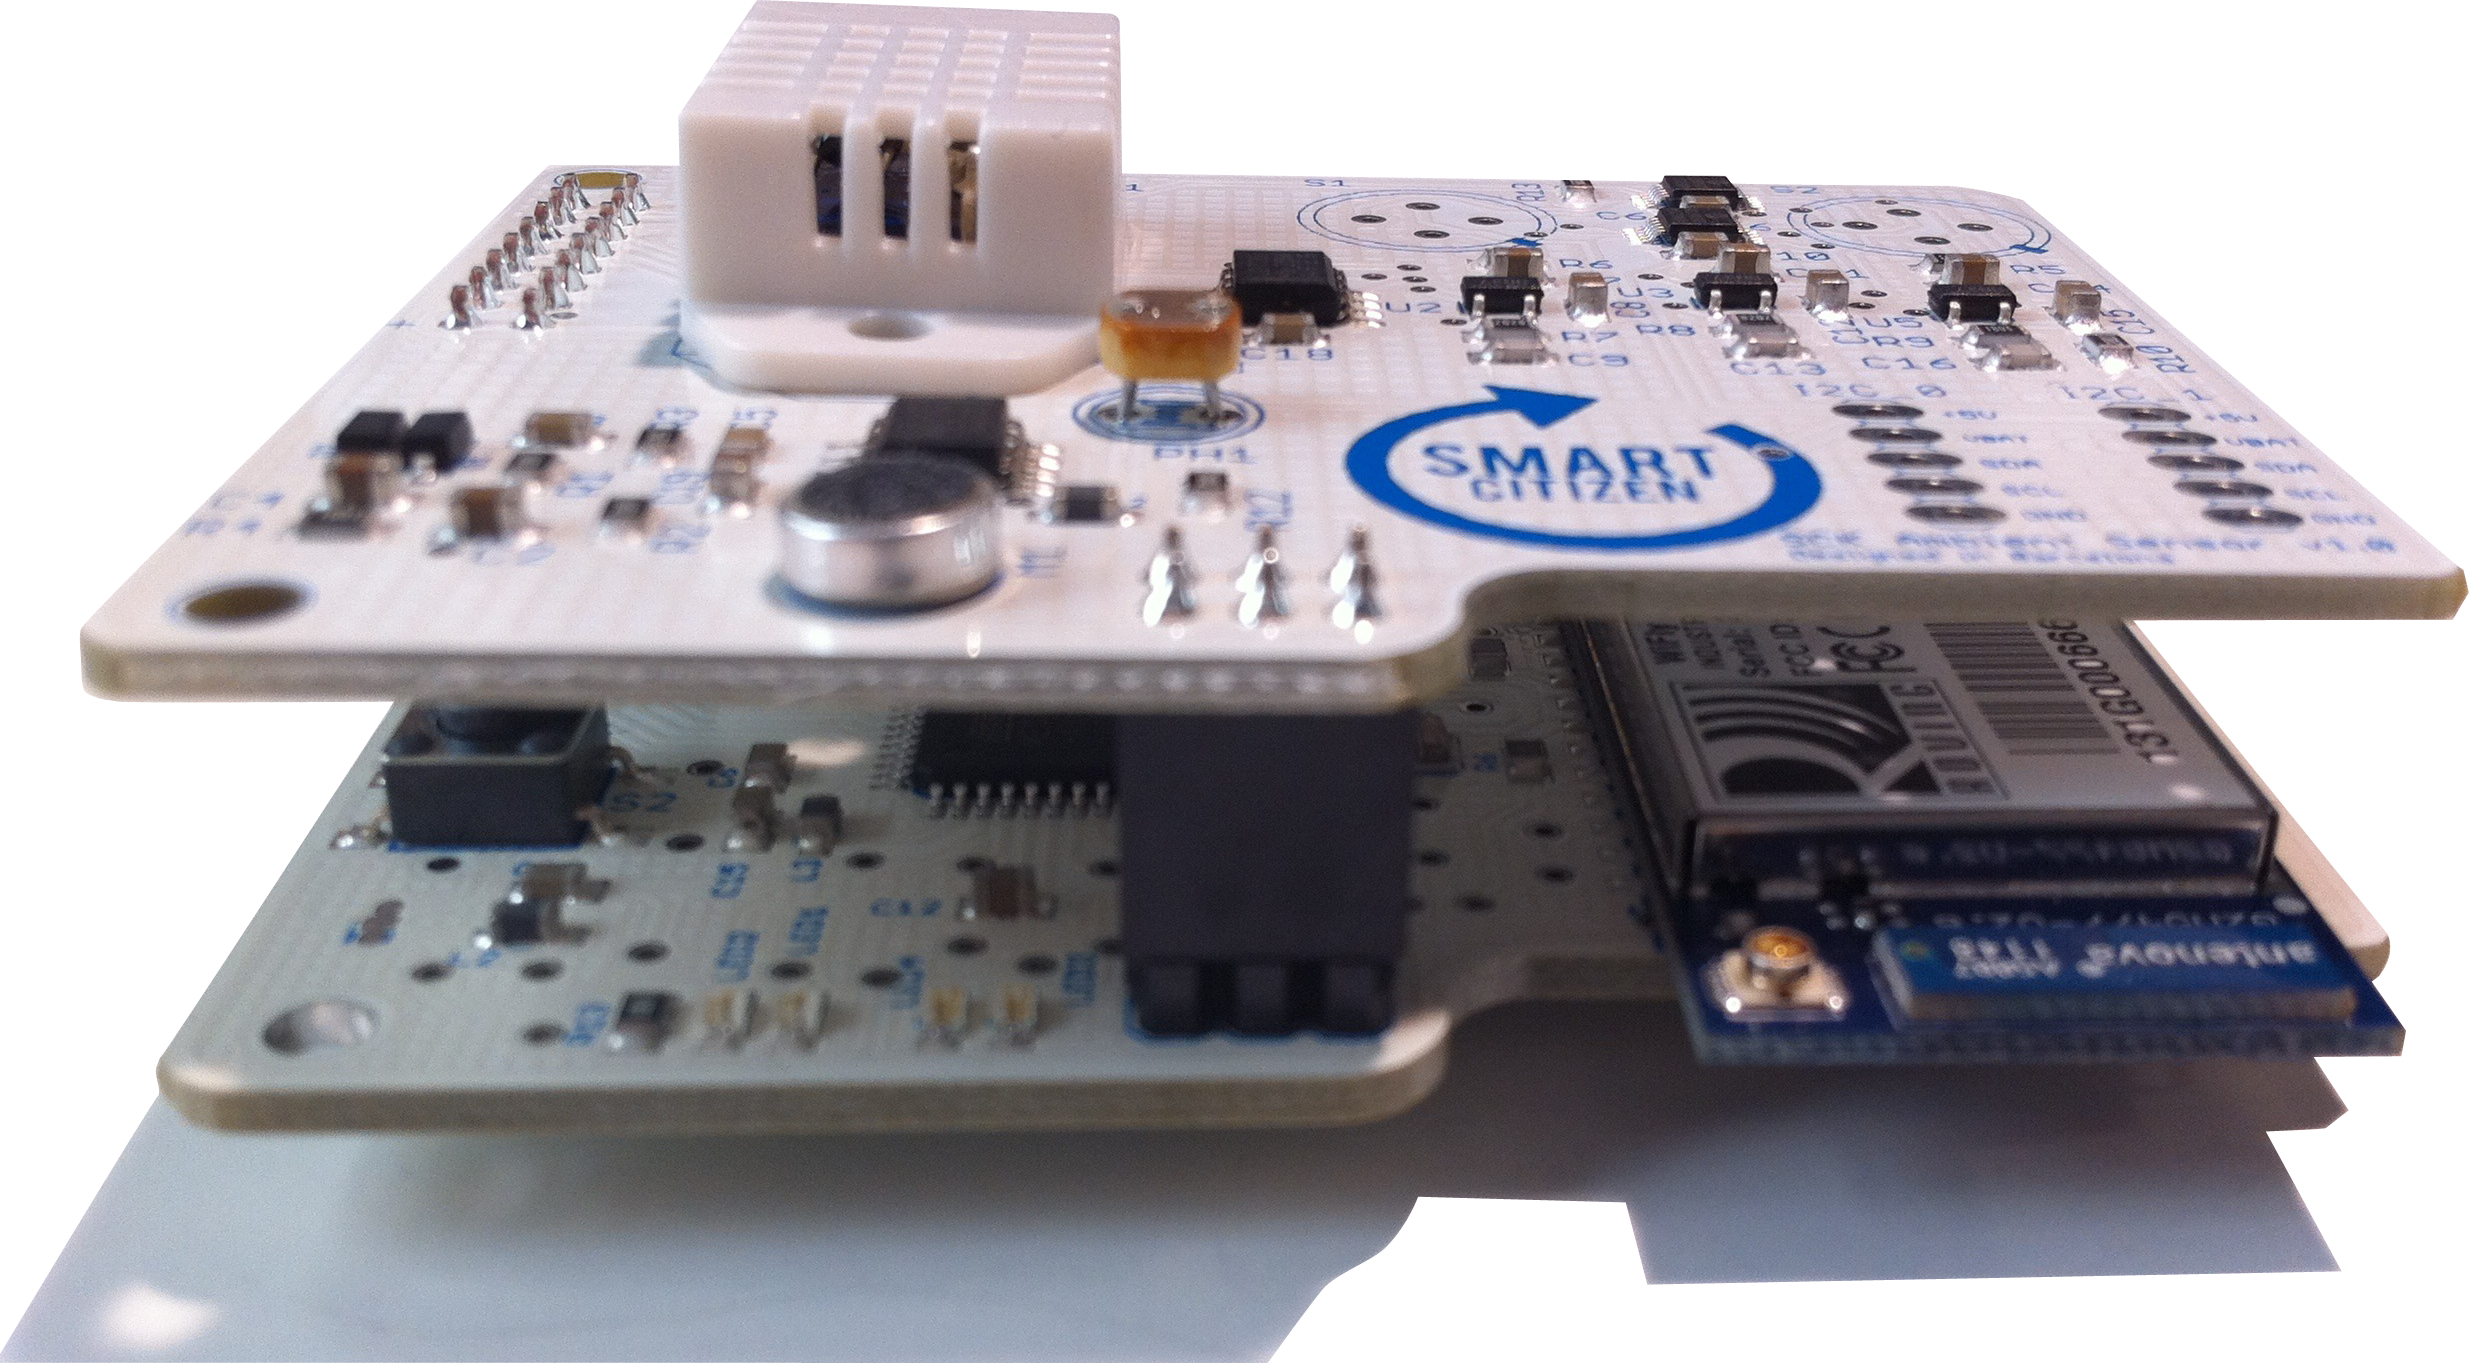
\includegraphics[scale=0.08]{./Figures/smartcitizen.png}
            \rule{18em}{0.5pt}
        \caption[Smart Citizen Node]{Smart Citizen Node.}
        \label{fig:SmartCitizenNode}
    \end{figure}
            
    \subsection{Libelium}
      Libelium is an ``Internet of things'' platform provider\footnote{\url{http://www.libelium.com/}}, which supplies an open source sensor platform for the Internet of things.
      They have a variety of products, some interesting ones are reported here:
      \begin{itemize}
        \item e-Health: A sensor shield for Arduino and Raspberry Pi for body monitoring: pulse, oxygen in blood, airflow (breathing), body temperature, electrocardiogram, glucometer, galvanic skin response, blood pressure, patient position, and muscle/electromyography sensor (Figure \ref{fig:Libeliumehealth}).
        
        \item Waspmote: A sensor node where it is possible attach more than 60 sensors, solar powered, and though to fit onto street light poles. (Figure \ref{fig:LibeliumWaspmote}).
       
       \item Smart Water: A Wireless Sensor Platform for water quality monitoring, it provides real-time data. (Figure \ref{fig:LibeliumSmartWater}).
     \end{itemize}
      
      \begin{figure}
        \centering
        \begin{subfigure}[b]{0.3\textwidth}
                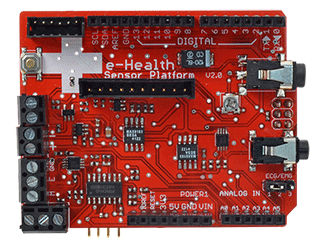
\includegraphics[width=\textwidth]{./Figures/Libeliume_health.png}
                \caption{Libelium ehealth}
                \label{fig:Libeliumehealth}
        \end{subfigure}%
        ~ %add desired spacing between images, e. g. ~, \quad, \qquad, \hfill etc.
          %(or a blank line to force the subfigure onto a new line)
        \begin{subfigure}[b]{0.3\textwidth}
                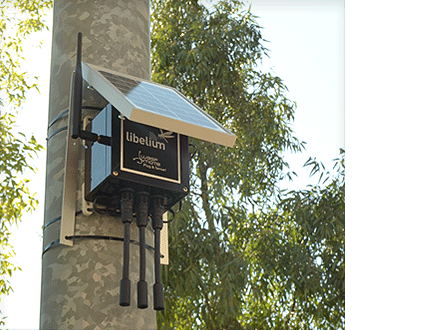
\includegraphics[width=\textwidth]{./Figures/LibeliumWaspmote.png}
                \caption{Libelium Waspmote}
                \label{fig:LibeliumWaspmote}
        \end{subfigure}
        \begin{subfigure}[b]{0.3\textwidth}
                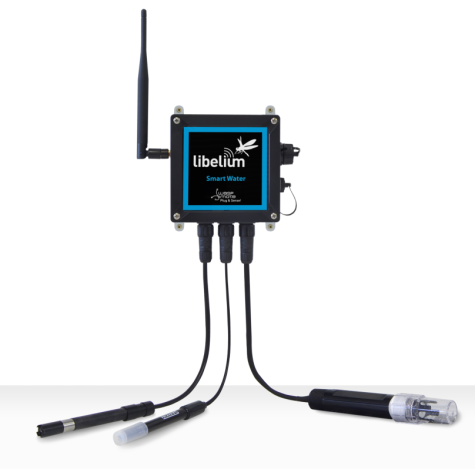
\includegraphics[width=\textwidth]{./Figures/LibeliumSmartWater.png}
                \caption{Libelium Smart Water}
                \label{fig:LibeliumSmartWater}
        \end{subfigure}
        \rule{18em}{0.5pt}
        \caption{Libellium Projects}\label{fig:LibelliumProjects}
		\end{figure}

  \section{Opendata services}
    The sensor boards are continuously collecting data which has to be stored. The data can be stored remotely or locally, but collecting it from every sensor board it is unpractical, for this reason an online storage service, Open data, is needed. The term Open data pursues the fact that certain types of data should be available to anyone, without any control mechanism, e.g. copyright.
    
		\subsection{Opencities}
       Opencities \cite{opencities} is a platform to browse, visualize, and download open data from different participants. Opencities has a very simple API to upload and download data, a web page to visualize the stored data.
       
    \subsection{Xively}
      Xively \footnote{\url{https://xively.com}} offers an Internet of Things platform as a service, basically it lets you store sensor data, download it, and visualize it through graphics.
    
    \subsection{Sentilo}
      Sentilo \footnote{\url{http://www.sentilo.io}} is an open source platform for Smart cities, it allows the user to use their own service to store the data, but they are not looking to be a database where everyone will store their sensor data, they want that each organization has its own sentilo server. The Sentilo platform does not depend on a central server and can be installed on a private server. It also provides an interface to show the data.
    
  \section{Sensor boards}
    In this section are discussed some of the options for a sensor node.
    
    \subsection{Arduino YUN}
      The Arduino YUN is a micro controller board with two processors (Figure \ref{fig:AYUN}), an ATmega32u4 (Arduino), and an Atheros AR9331 (Which runs a Linux distribution named OpenWrt-Yun). It has an Ethernet and WiFi module, a USB-A port, a micro-SD card slot, 20 digital input/output ping, 16 MHz crystal oscillator, ICSP header, and 3 reset buttons.
      \begin{figure}[htbp]
        \centering
            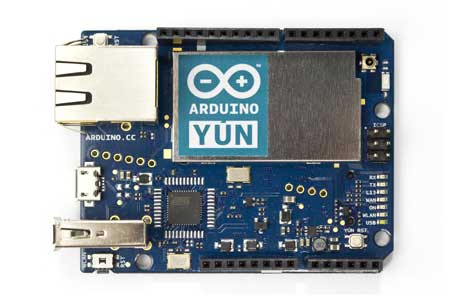
\includegraphics[scale=0.4]{./Figures/ArduinoYunFront_2_450px.jpg}
            \\
            \rule{15em}{0.5pt}
        \caption[Arduino YUN]{Arduino YUN.}
        \label{fig:AYUN}
      \end{figure}
      
      The peculiarity about the Arduino YUN is that the processor for the Arduino sketches can communicate with the Linux processor through the bridge library (Figure \ref{fig:BridgeInShort}), which allows to write Python scripts and execute them.
      
      A Power over Ethernet module (PoE) can be attach to the Arduino, which has a particular interest for the Guifi network, where the antennas are powered through PoE.
      \begin{figure}[htbp]
          \centering
              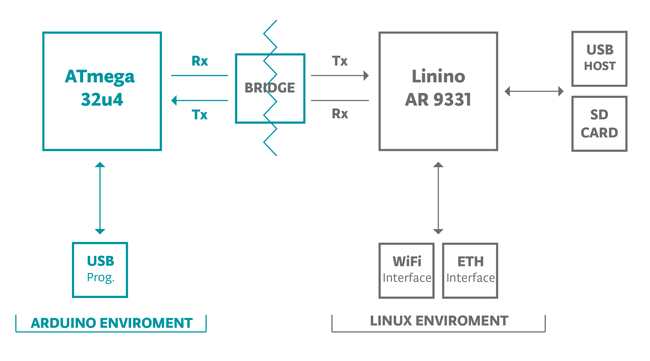
\includegraphics[scale=0.5]{./Figures/BridgeInShort.png}
              \\
              \rule{23em}{0.5pt}
          \caption[Arduino YUN Bridge]{Arduino YUN Bridge.}
          \label{fig:BridgeInShort}
       \end{figure}
        
    \subsection{Raspberry Pi}
      Raspberry Pi\footnote{\url{http://www.raspberrypi.org/}} is a single-board computer, produced in two models, A and B. The model B (Figure \ref{fig:RaspberryPiB}) is more appropriate for this project because it has an Ethernet controller. It is composed by an HDMI, a micro USB, an USB 2.0 connector, an SD card slot, Input/Output (GPIO) pins, an RCA connector, an audio jack, an Ethernet controller, and a Broadcom BCM2835 processor.
     
      It is possible to attach sensors to it, and it supports Linux environment.
      \begin{figure}[htbp]
          \centering
              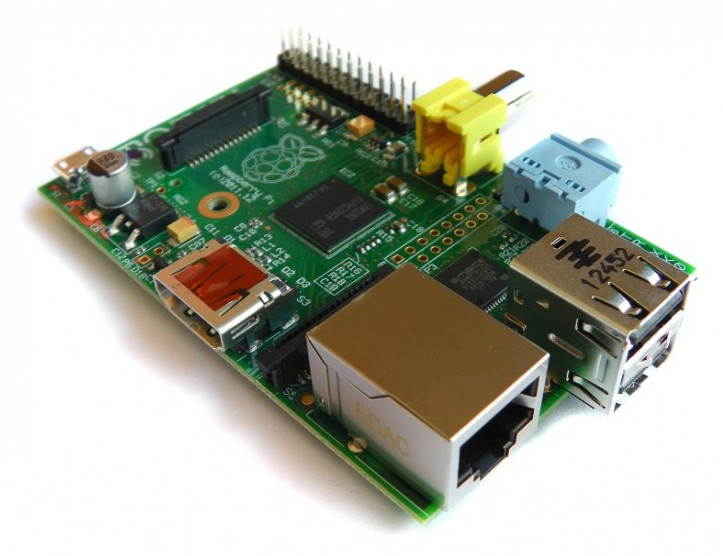
\includegraphics[scale=0.2]{./Figures/raspberry-pi-model-b.jpg}
              \\
              \rule{15em}{0.5pt}
          \caption[Raspberry Pi model B]{Raspberry Pi model B.}
          \label{fig:RaspberryPiB}
       \end{figure}
    
    \subsection{Picoboard}      
      PicoBoard\footnote{\url{http://www.picocricket.com/picoboard.html}} (Figure \ref{fig:picoboard}) is a board to interact with the world, it can be programmed by Scratch projects. It is less flexible than the previously mentioned, it is composed by a button, a light and a sound sensor, a slider, and alligator clips which can be use to connect custom sensors.
      
      \begin{figure}[htbp]
          \centering
              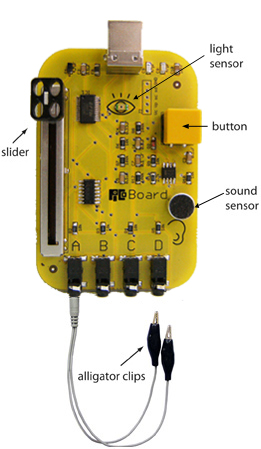
\includegraphics[scale=0.5]{./Figures/picoboard.jpg}
              \\
              \rule{16em}{0.5pt}
          \caption[Picoboard]{Picoboard.}
          \label{fig:picoboard}
       \end{figure}

\chapter{Technologies}
\label{Chapter3}
  
  This chapter is focused on the technologies used to develop this project.
  
  \section{Arduino-Raspberry PI comparison}
  
  	Sensor networks should not affect the environment, in our case, visually. For this purpose we must ensure that the nodes are relatively small, so the board and sensors had been selected accordingly.
    
    To choose the processor board, have been considered the following characteristics:
    
    \begin{itemize}
    	\item {\bf Power:} A sensor node can obtain energy in several ways: batteries, solar energy, connecting to an already deployed network, etc. The important thing is not to increase the size of the sensor node, in our case, the power is given by an already deployed network.
    	\item {\bf CPU:} A powerful CPU is not necessary to process sensor data, so this helps to decrease the size of the board and reduce power consumption.
    	\item {\bf Communication:} The collected data has to be sent to the broker, usually through a wireless or wired network. If the communication is wireless, the topology and location of the sensor nodes has to be chosen properly. But if the connection is through a wired network, it should take advantage of something already deployed, in our case, the Guifi network.
    \end{itemize}
    
    For this project, two possible boards have been considered: the Arduino Yun (Yun) and the Raspberry Pi model B (RPiB). The Yun is a microcontroller while the RPiB is a full computer, which makes it more powerful, even more than needed.
    
    The two of them have a Linux environment, but with the Yun, the normal way to interact is by an Arduino sketch. RPiB considers that the developer has some prior Linux knowledge, while the Yun is better for beginners. Also, the Arduino IDE provides a variety of programs that help the learning process.
    
    Another difference is that Arduino is open hardware, which might be helpful if it has to be improved.
    
    The sensor board is the biggest element of the sensor node, so the size is very important, the smaller the better. In this case, the Yun is smaller than the RPiB. On the other hand, the sensor node will be attach to Guifi nodes, which are powered by Power over Ethernet (PoE). 
    For the Yun there is the possibility to connect a PoE module (not available yet), which will power the board. The Figure \ref{fig:arduinoethernetpoe} and \ref{fig:poerpi} show the comparison between the size of an Arduino Ethernet (similar to the YUN) and the RPiB both powered by PoE. It is clearly visible that the Arduino is more compact.
    
    \begin{figure}
        \centering
        \begin{subfigure}[b]{0.3\textwidth}
                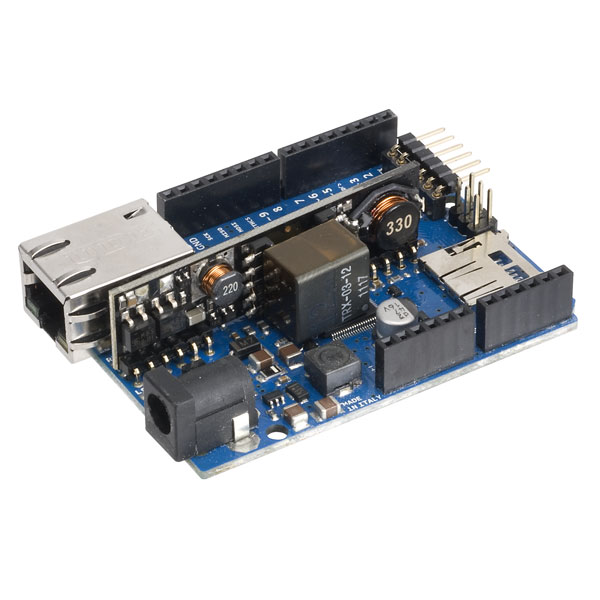
\includegraphics[width=\textwidth]{./Figures/arduinoethernetpoe.jpg}
                \caption{Arduino Ethernet PoE}
                \label{fig:arduinoethernetpoe}
        \end{subfigure}%
        ~ %add desired spacing between images, e. g. ~, \quad, \qquad, \hfill etc.
          %(or a blank line to force the subfigure onto a new line)
        \begin{subfigure}[b]{0.3\textwidth}
                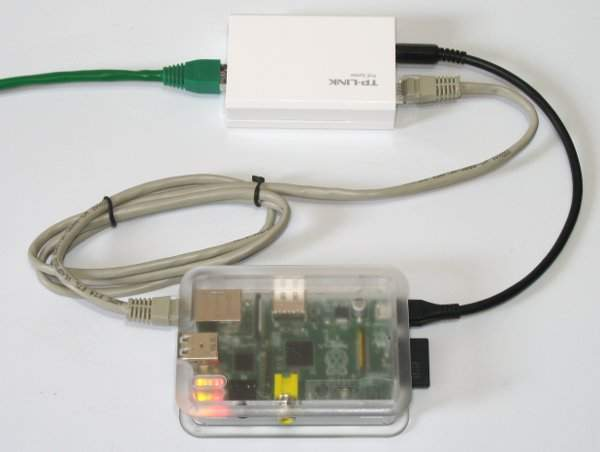
\includegraphics[width=\textwidth]{./Figures/poe-rpi.jpg}
                \caption{Raspberry Pi (B) PoE}
                \label{fig:poerpi}
        \end{subfigure}
        \rule{18em}{0.5pt}
        \caption{Sensor boards}\label{fig:sensorboards}
		\end{figure}

    Another advantage that YUN offers is the integrated WiFi module, which offers more flexibility when there is no ethernet available.
    
    Finally, the YUN has been used instead of the RPiB basically because of the size that will become the sensor node, but if in the future will be necessary a more powerful processor, the RPiB is better suited.
    
    The Table \ref{tab:YUN-RPiBcomparisonfig:sensorboards} shows the differences between the RPiB and the YUN explained before.
    
    \begin{table}
    	\centering
		  \begin{tabular}{ | l | p{6cm} | p{3cm} |}
				\hline
				{\bf Functionalities} & {\bf YUN} & {\bf RPiB} \\ \hline
				Way of interaction & Arduino Sketch and Linux & Linux \\ \hline
				Development skills required & Low skills with Arduino and Linux & Medium skills \\ \hline
				Size of the board & 6.58 x 5.33 cm & 8.55 x 5.41 cm \\ \hline
				Computational power & Yun:16MHz - Linux:400MHz & 700MHz \\ \hline
				Available memory & Yun: 32 KB - Linux: 16 MB & 512MB \\ \hline
		  \end{tabular}
      \caption{YUN-RPiB comparison}
      \label{tab:YUN-RPiBcomparisonfig:sensorboards}
		\end{table}

  \section{Sensors}
    The goal is to analyze the environment around us, and sensors are a meant to detect physical or chemical variables. It has been decided to use low cost environmental sensors that are easily accessible and usable. 
    These sensors measure the aspects that may be more useful for citizens: temperature, light, noise, humidity, and air quality.
    
    A sensor is a device which transform a physical measure to an output signal (Voltage or Digits) that can be read by another device, such as an Arduino.
    In this project five sensors has been used to measure temperature, light, noise, humidity, and gas.
    To show how the sensors are connected to the Arduino YUN the program Fritzing\footnote{\url{http://fritzing.org/}} has been used.
    
    \subsection{LM35: Temperature}
      LM35 [Figure \ref{fig:LM35}] is a sensor to measure temperature, in the Figure \ref{fig:TemperatureSensor_bb} is shown how to connect it to the Arduino.
      \cite{LM35}
      
      \begin{figure}
        \centering
        \begin{subfigure}[b]{0.3\textwidth}
                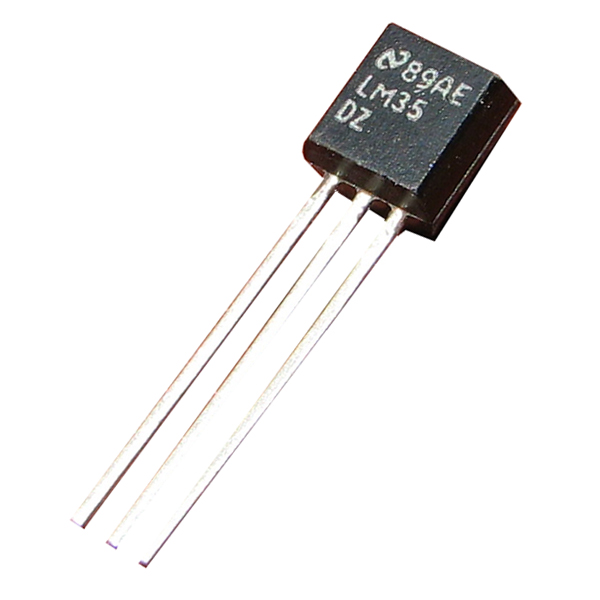
\includegraphics[width=\textwidth]{./Figures/LM35.jpg}
                \caption{LM35 sensor}
                \label{fig:LM35}
        \end{subfigure}%
        ~ %add desired spacing between images, e. g. ~, \quad, \qquad, \hfill etc.
          %(or a blank line to force the subfigure onto a new line)
        \begin{subfigure}[b]{0.3\textwidth}
                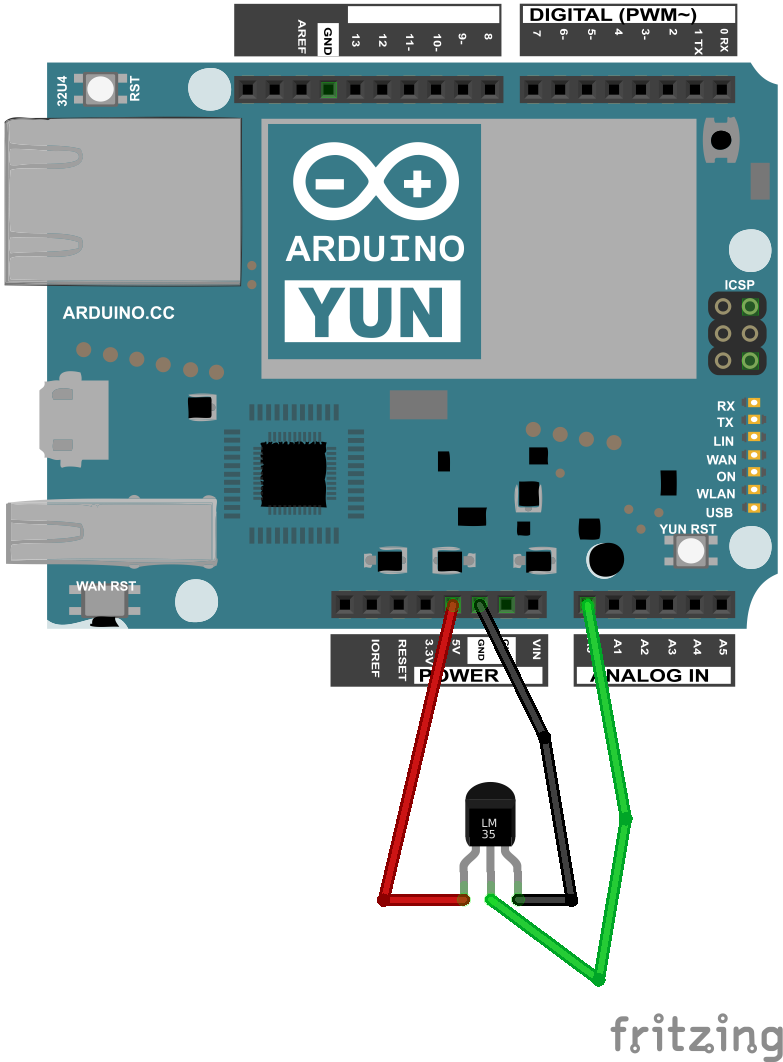
\includegraphics[width=\textwidth]{./Figures/Fritzing/TemperatureSensor_bb.png}
                \caption{Temperature Sensor Breadboard}
                \label{fig:TemperatureSensor_bb}
        \end{subfigure}
        \rule{18em}{0.5pt}
        \caption{Temperature sensor}\label{fig:temperaturesensor}
		\end{figure}
      
    \subsection{Light Dependent Resistor (LDR)}
      LDR [Figure \ref{fig:LDR}] is a light sensor, in the Figure \ref{fig:LightSensor_bb} is depicted how to connect it to the Arduino.
      
      \begin{figure}
        \centering
        \begin{subfigure}[b]{0.3\textwidth}
                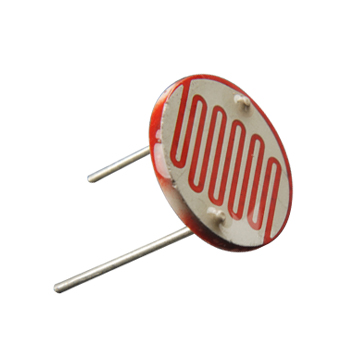
\includegraphics[width=\textwidth]{./Figures/LDR.jpg}
                \caption{LDR sensor}
                \label{fig:LDR}
        \end{subfigure}%
        ~ %add desired spacing between images, e. g. ~, \quad, \qquad, \hfill etc.
          %(or a blank line to force the subfigure onto a new line)
        \begin{subfigure}[b]{0.3\textwidth}
                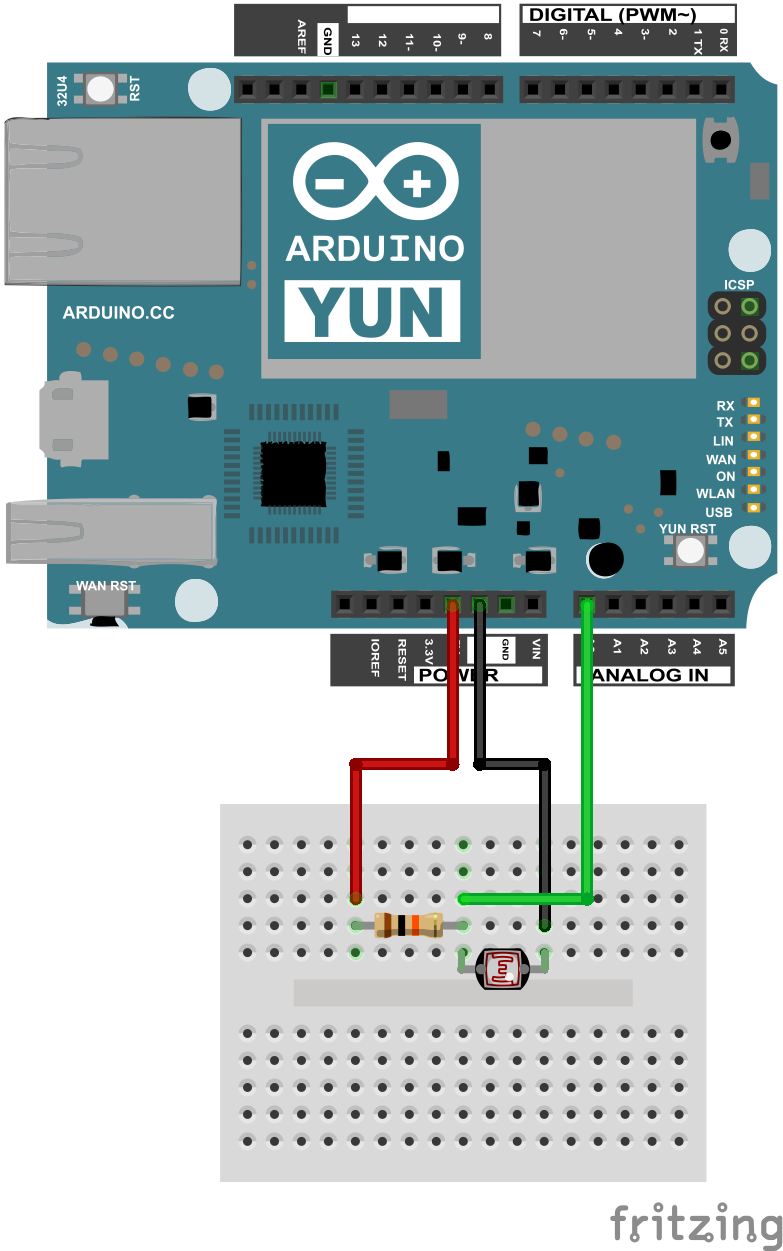
\includegraphics[width=\textwidth]{./Figures/Fritzing/LightSensor_bb.png}
                \caption{Light Sensor Breadboard}
                \label{fig:LightSensor_bb}
        \end{subfigure}
        \rule{18em}{0.5pt}
        \caption{Light sensor}\label{fig:lightsensor}
			\end{figure}
 
    \subsection{Emartee Mini Sound Sensor and Analog Sound Sensor Board Microphone MIC Controller: Noise}
      This two sensors \cite{emarteeminisound} are used to measured noise levels [Figure \ref{fig:MSS}] and [Figure \ref{fig:Analognoisesensor}]. The code to read the noise values is the same for both. In the Figure \ref{fig:NoiseSensor_bb} is shown how to connect them to the Arduino.
      
      \begin{figure}
        \centering
        \begin{subfigure}[b]{0.3\textwidth}
                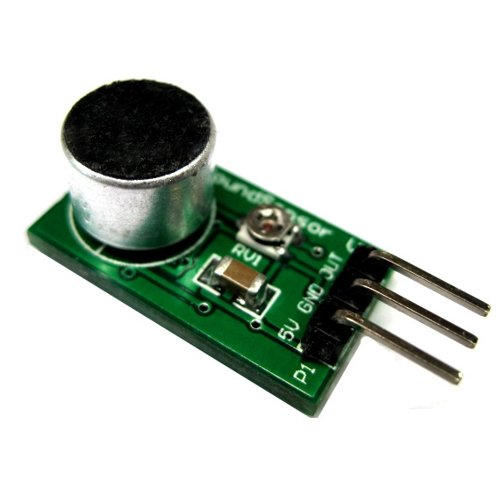
\includegraphics[width=\textwidth]{./Figures/MiniSoundSensor.jpg}
                \caption{Mini Sound Sensor}
                \label{fig:MSS}
        \end{subfigure}%
        ~ %add desired spacing between images, e. g. ~, \quad, \qquad, \hfill etc.
          %(or a blank line to force the subfigure onto a new line)
        \begin{subfigure}[b]{0.3\textwidth}
                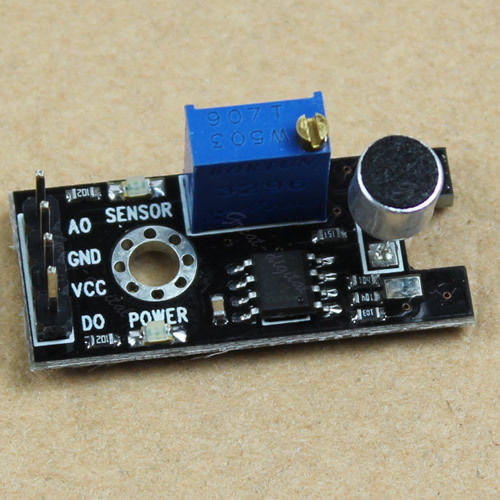
\includegraphics[width=\textwidth]{./Figures/analognoisesensor.jpg}
                \caption{Analog noise sensor}
                \label{fig:Analognoisesensor}
        \end{subfigure}
        \begin{subfigure}[b]{0.3\textwidth}
                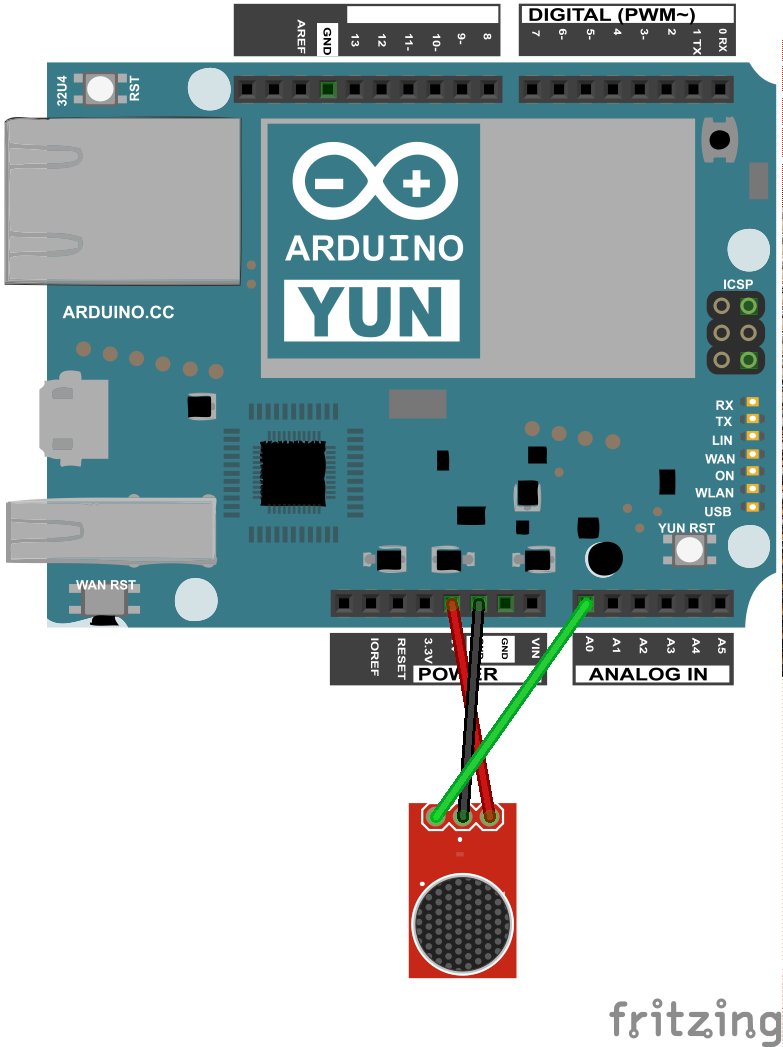
\includegraphics[width=\textwidth]{./Figures/Fritzing/NoiseSensor_bb.png}
                \caption{Noise Sensor Breadboard}
                \label{fig:NoiseSensor_bb}
        \end{subfigure}
        \rule{35em}{0.5pt}
        \caption{Noise sensor}\label{fig:noisesensor}
			\end{figure}


    \subsection{Aosong DHT22 and DHT11: Humidity}
      DHT22 [Figure \ref{fig:DHT22}] and DHT11 [Figure \ref{fig:DHT11}] are humidity and temperature sensors, although the humidity measure is the only one used. The output is digital, and to read it, an external library\footnote{\url{https://github.com/adafruit/DHT-sensor-library}} is needed. The Arduino and the humidity sensor have to be connected as shown in the Figure \ref{fig:HumiditySensordht22_bb} for the DHT22 and as shown in the Figure \ref{fig:HumiditySensordht11_bb} for the DHT11 \cite{dht22sensor}.
      
      \begin{figure}
        \centering
        \begin{subfigure}[b]{0.3\textwidth}
                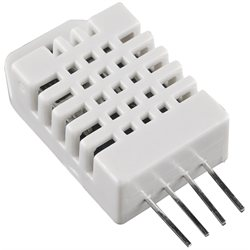
\includegraphics[width=0.8\textwidth]{./Figures/dht22.jpg}
                \caption{DHT22 sensor}
                \label{fig:DHT22}
        \end{subfigure}%
        ~ %add desired spacing between images, e. g. ~, \quad, \qquad, \hfill etc.
          %(or a blank line to force the subfigure onto a new line)
        \begin{subfigure}[b]{0.3\textwidth}
                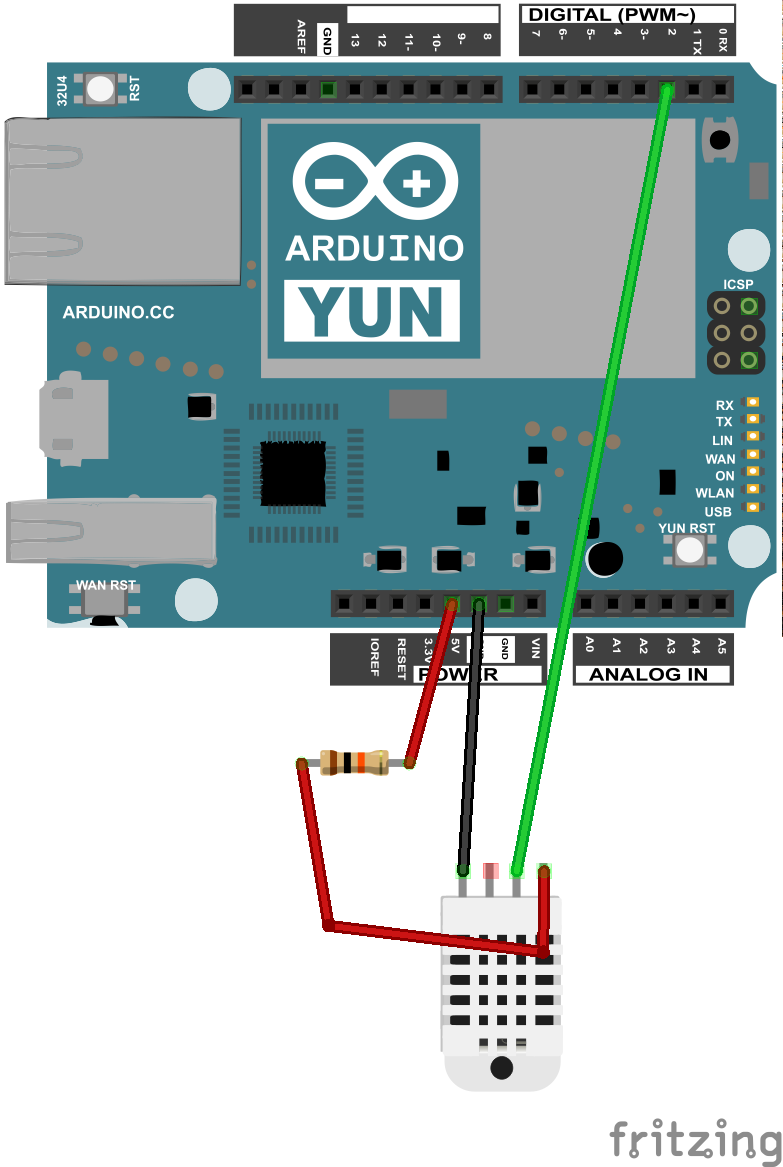
\includegraphics[width=\textwidth]{./Figures/Fritzing/HumiditySensor_bb.png}
                \caption{DHT22 Sensor Breadboard}
                \label{fig:HumiditySensordht22_bb}
        \end{subfigure}
        \rule{18em}{0.5pt}
        \caption{DHT22 sensor}\label{fig:DHT22sensor}
			\end{figure}
      
      \begin{figure}
        \centering
        \begin{subfigure}[b]{0.3\textwidth}
                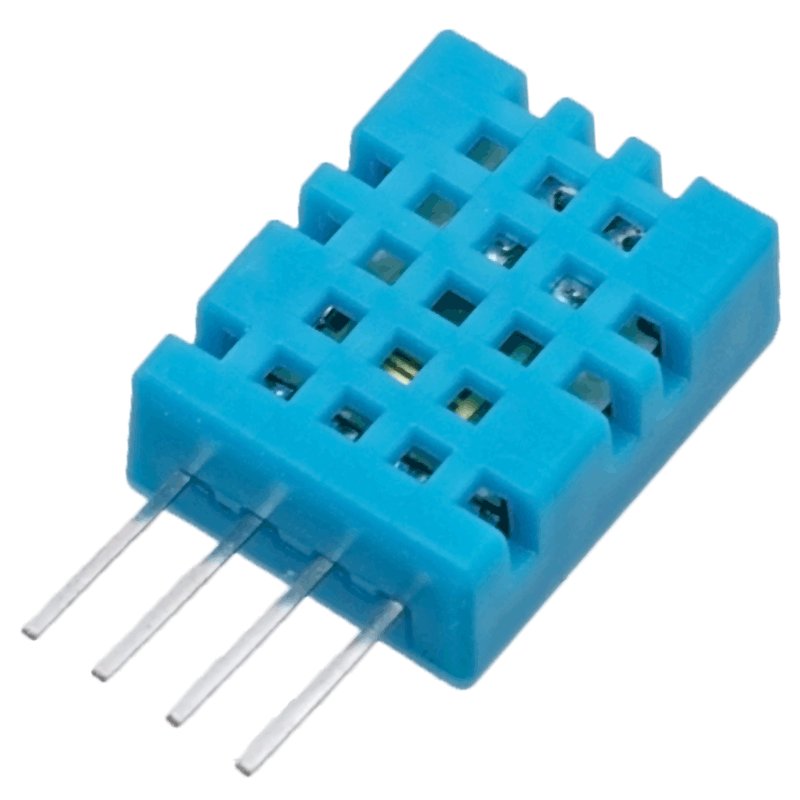
\includegraphics[width=0.7\textwidth]{./Figures/dht11.png}
                \caption{DHT11 sensor}
                \label{fig:DHT11}
        \end{subfigure}%
        ~ %add desired spacing between images, e. g. ~, \quad, \qquad, \hfill etc.
          %(or a blank line to force the subfigure onto a new line)
        \begin{subfigure}[b]{0.3\textwidth}
                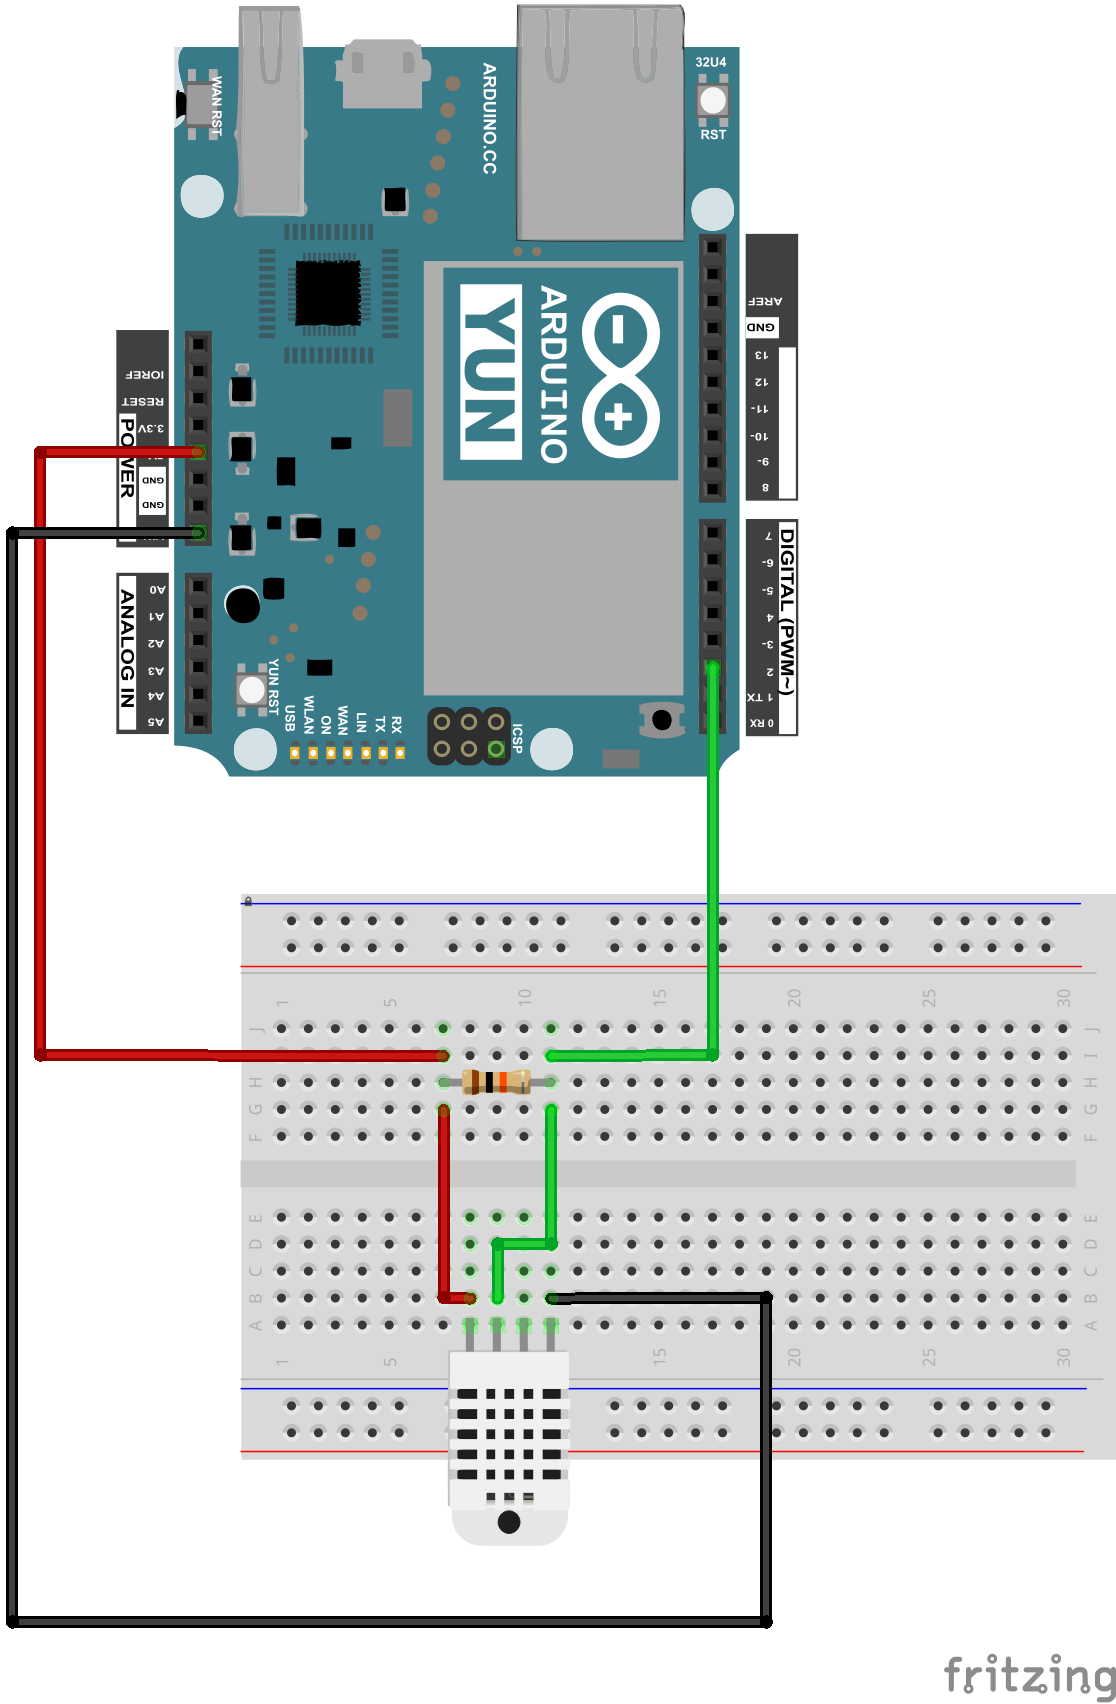
\includegraphics[width=\textwidth]{./Figures/Fritzing/HumiditySensorDht11_bb.png}
                \caption{DHT11 Sensor Breadboard}
                \label{fig:HumiditySensordht11_bb}
        \end{subfigure}
        \rule{18em}{0.5pt}
        \caption{DHT11 sensor}\label{fig:DHT11sensor}
			\end{figure}     
      
    \subsection{MQ135: Gas sensor}
      MQ135 is a gas sensor [Figure \ref{fig:MQ135}], and is used to measure air quality. Figure \ref{fig:GasSensor_bb} illustrates how to connect it to the Arduino.      
      \begin{figure}
        \centering
        \begin{subfigure}[b]{0.3\textwidth}
                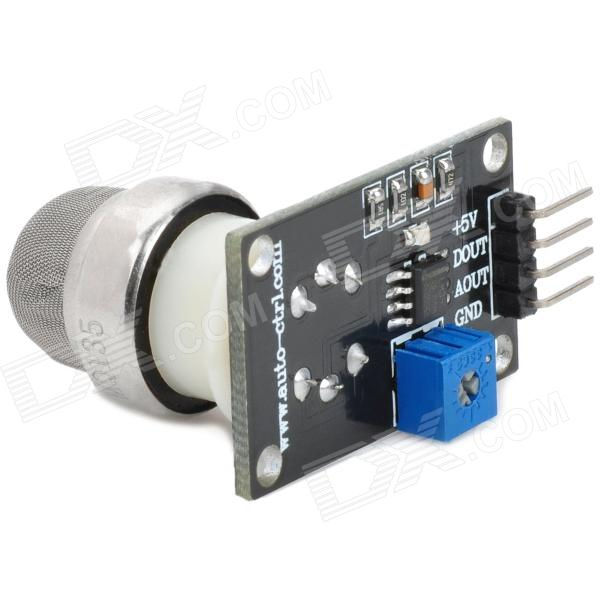
\includegraphics[width=0.7\textwidth]{./Figures/mq135.jpg}
                \caption{MQ135 Air Quality sensor}
                \label{fig:MQ135}
        \end{subfigure}%
        ~ %add desired spacing between images, e. g. ~, \quad, \qquad, \hfill etc.
          %(or a blank line to force the subfigure onto a new line)
        \begin{subfigure}[b]{0.3\textwidth}
                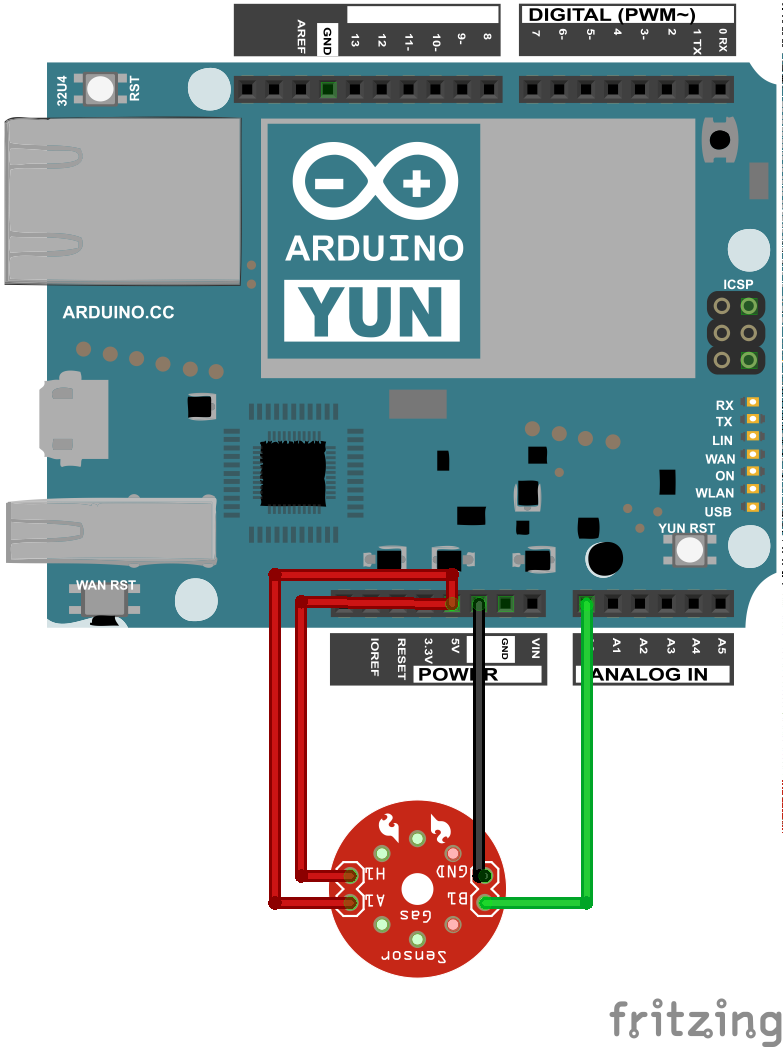
\includegraphics[width=\textwidth]{./Figures/Fritzing/GasSensor_bb.png}
                \caption{Gas Sensor Breadboard}
                \label{fig:GasSensor_bb}
        \end{subfigure}
        \rule{18em}{0.5pt}
        \caption{Gas sensor}\label{fig:DHT11sensor}
			\end{figure} 
      
      The Mq135 sensor reacts to the concentration of the following gases: NH3, NOx, alcohol, Benzene, smoke, CO2, etc. \cite{mq135gassensor}.
      
    \subsection{BreadBoard with all the sensors}
      
      In the Figure \ref{fig:AllSensors22_bb} is shown the final prototype with the DHT22 sensor, and in the Figure \ref{fig:AllSensors11_bb} with the DHT11 sensor.
      
      \begin{figure}[!htbp]
          \centering
              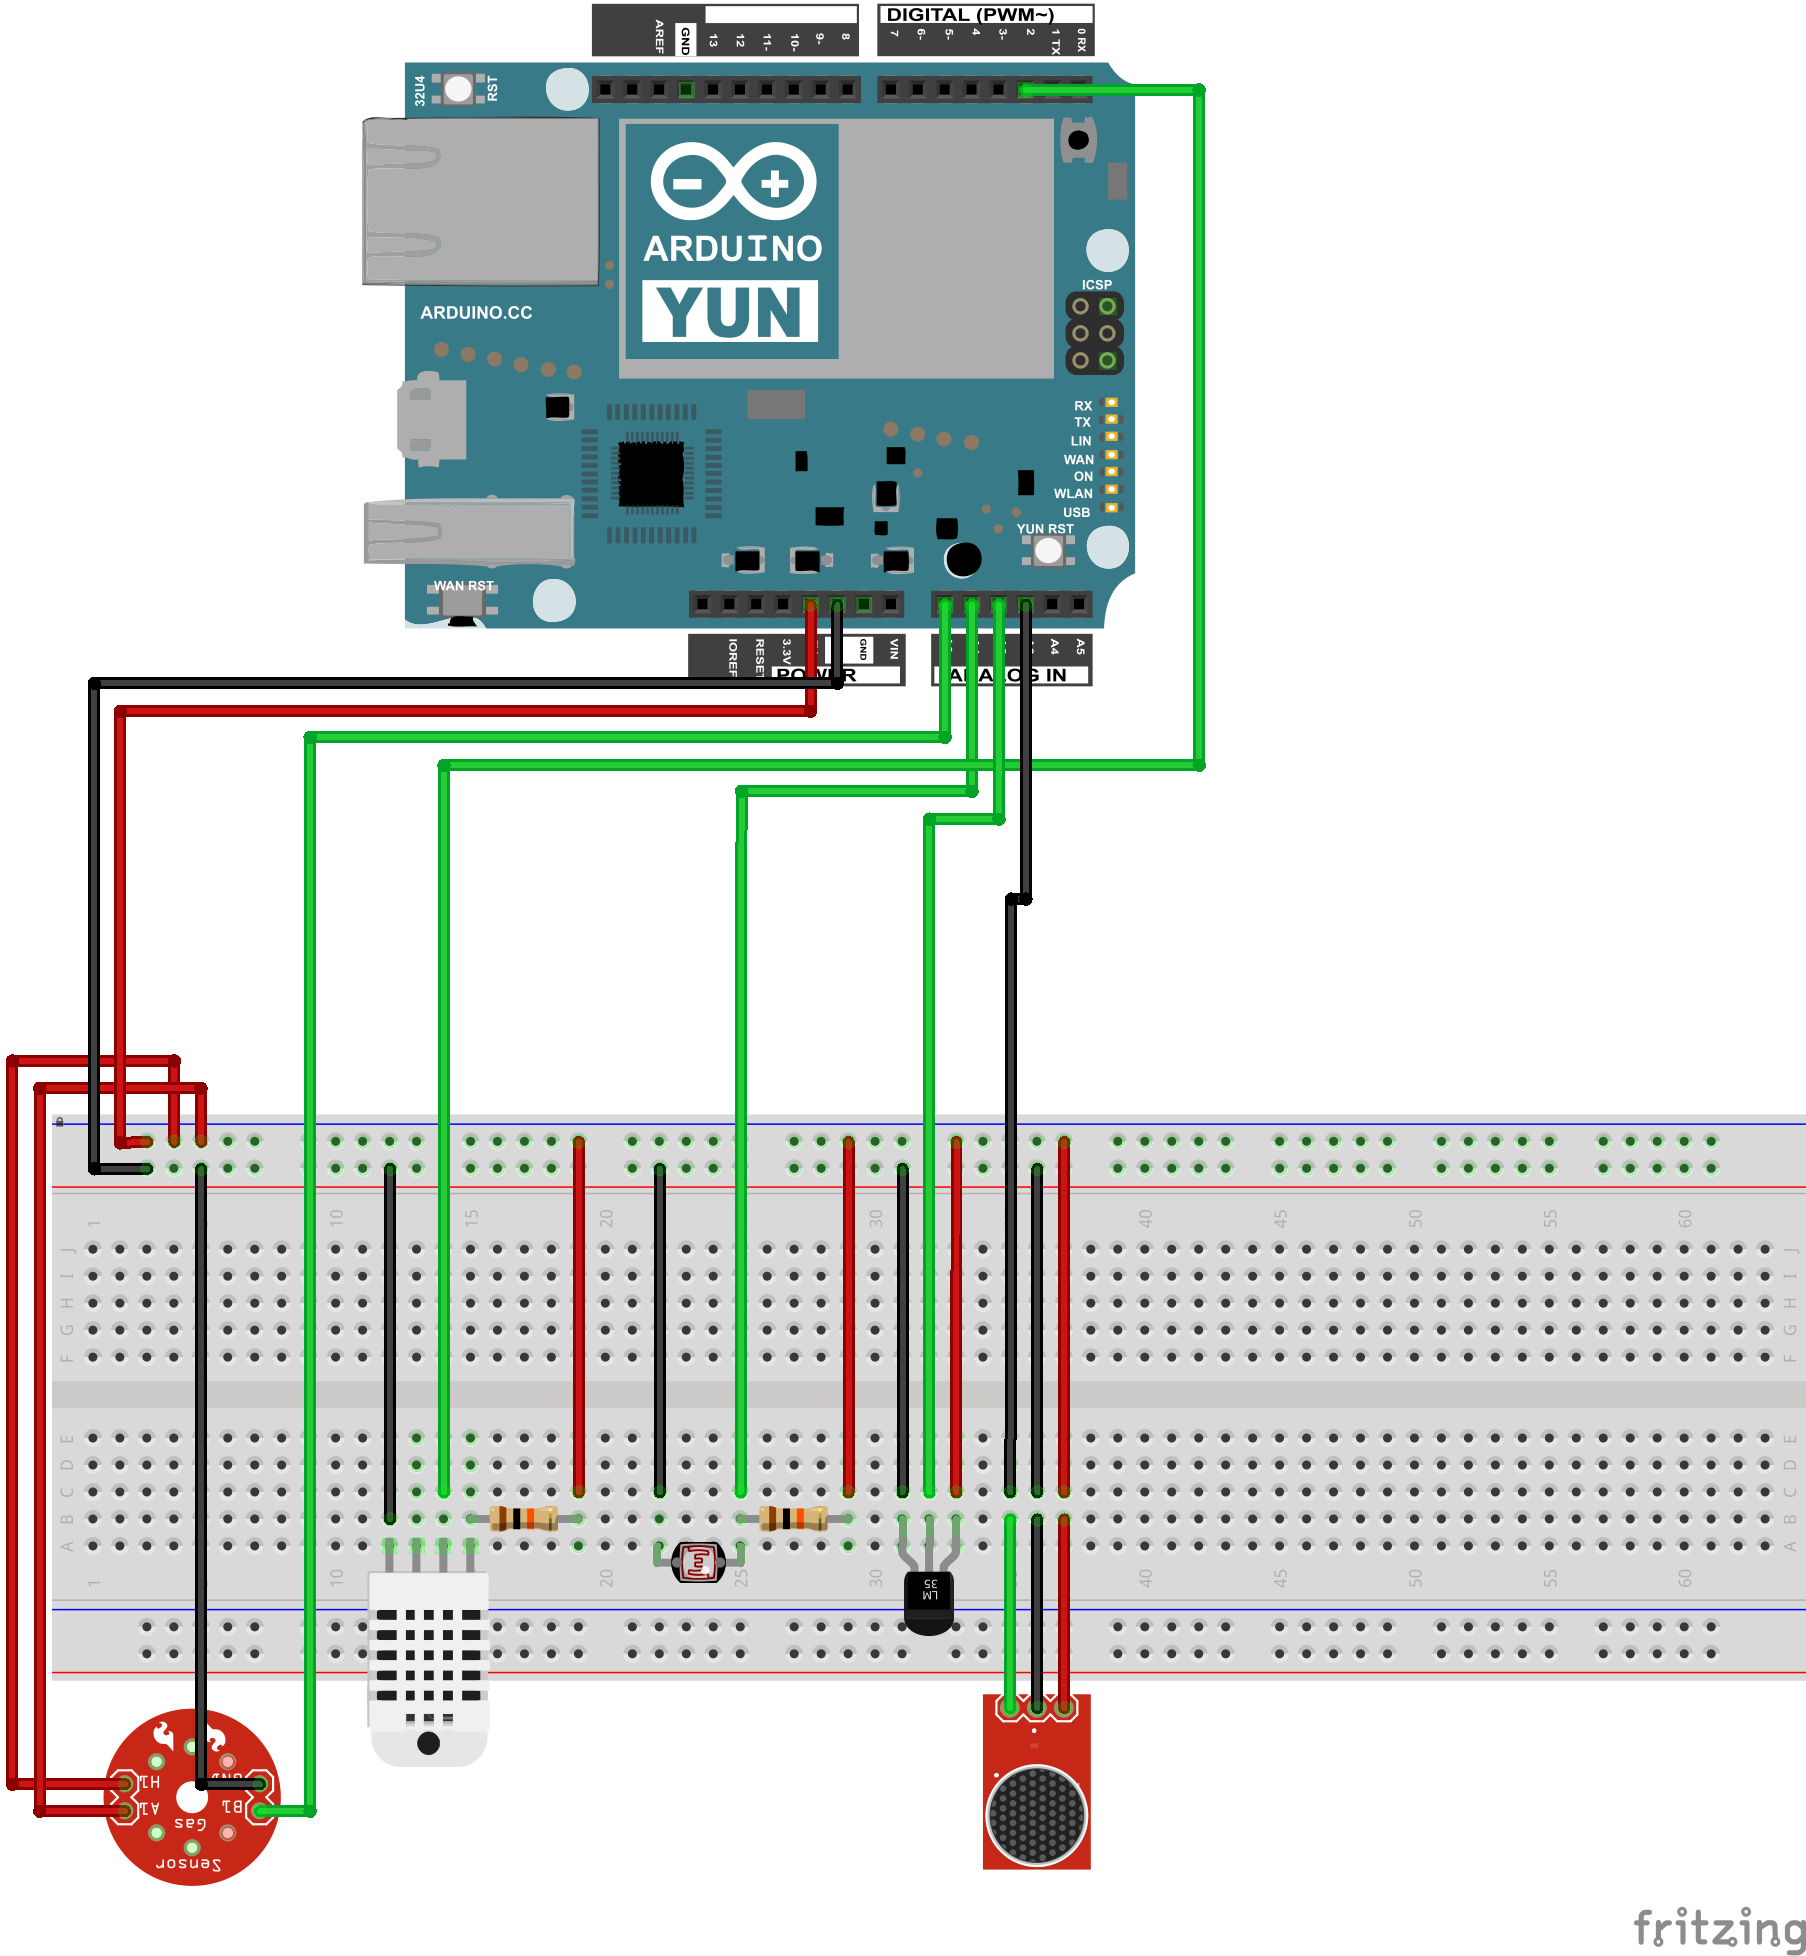
\includegraphics[scale=0.8]{./Figures/Fritzing/AllSensors22_bb.png}
              \rule{25em}{0.5pt}
          \caption[Sensor node Prototype with DHT22]{Sensor node Prototype with DHT22.}
          \label{fig:AllSensors22_bb}
      \end{figure}
      
      \begin{figure}[!htbp]
          \centering
              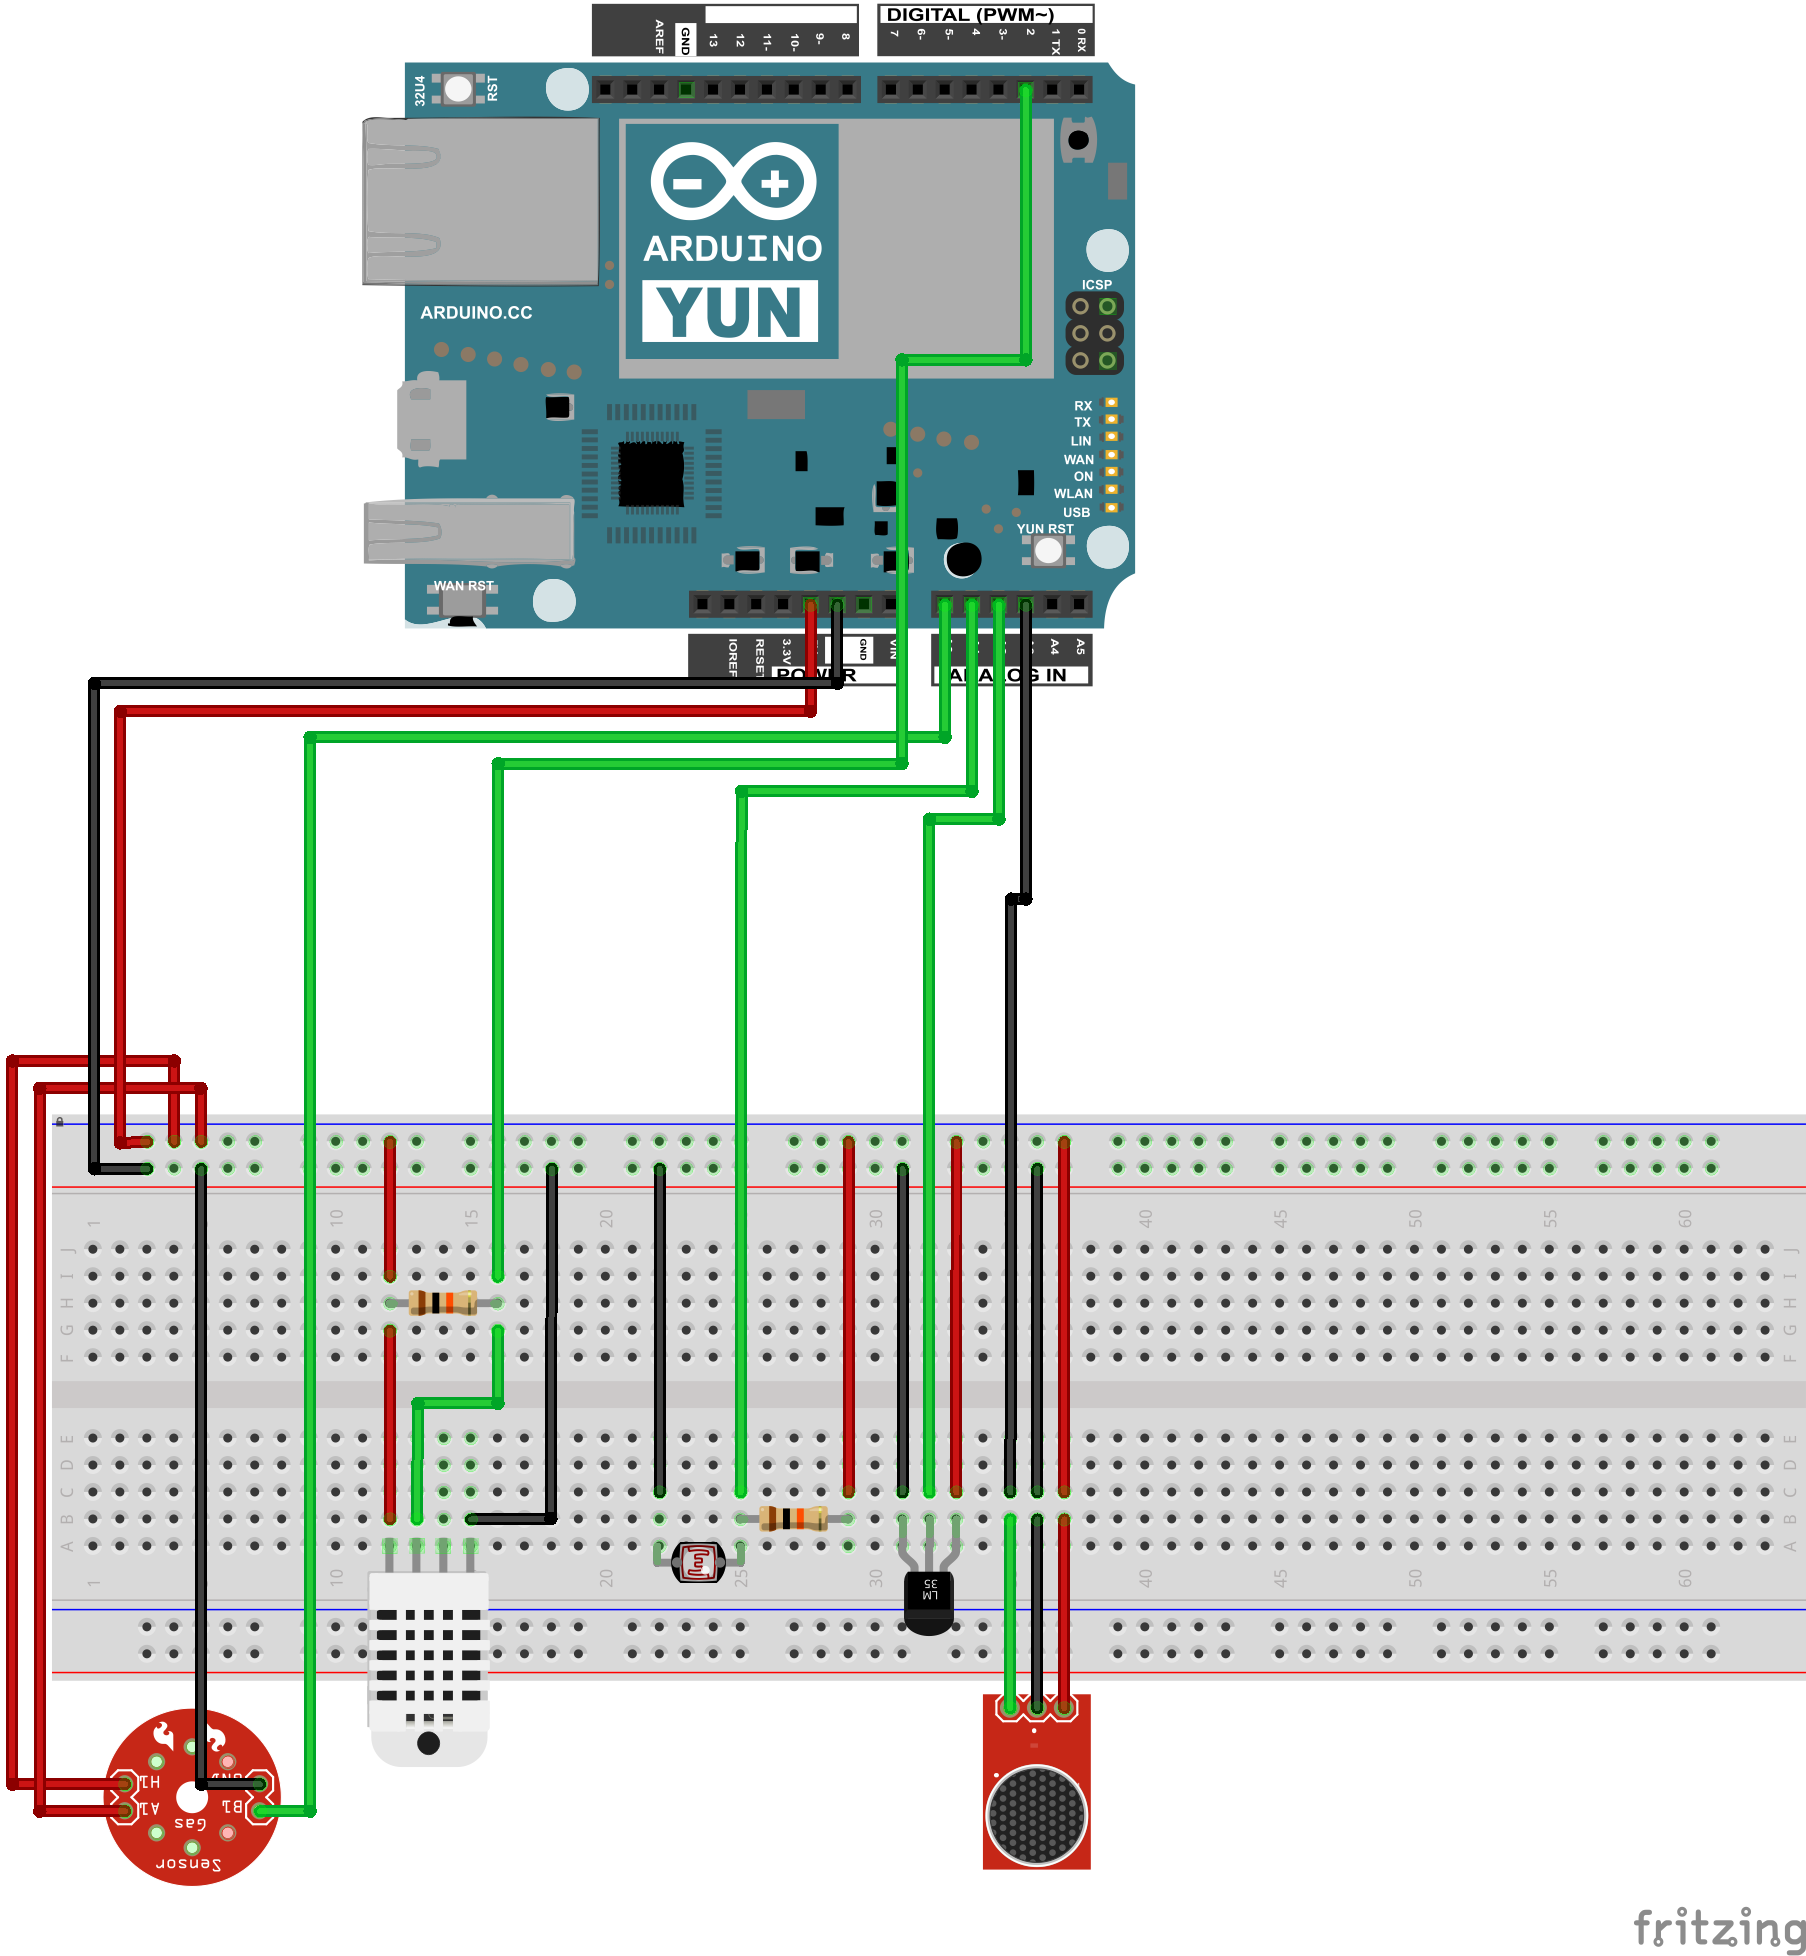
\includegraphics[scale=0.8]{./Figures/Fritzing/AllSensors11_bb.png}
              \rule{25em}{0.5pt}
          \caption[Sensor node Prototype with DHT11]{Sensor node Prototype with DHT11.}
          \label{fig:AllSensors11_bb}
      \end{figure}
    
  \section{Upload sensor data}
  
    A main part of the project is uploading the data from the sensors to a platform to make the data publicly available.
    
    The GeoJSON message (explained in section \ref{GeoJSON}) includes data from 5 sensors, which makes its size too large for the memory of the Arduino.
    For this type of operations is possible to run a script in the Linux environment through the Bridge library (Figure \ref{fig:BridgeInShort}).
    
    This being the path that is followed, there are several options for developing this script, for example Java, C / C + +, Python, etc..
    Python has been used because of the following reasons: fast and perfect for prototyping programming, the code is shorter and therefore, easier to understand, and modular.
    
    \subsection{GeoJSON}
    \label{GeoJSON}
      A GeoJSON\footnote{\url{http://geojson.org/}} is a format for encoding a variety of geographic data structures. The GeoJSON that has been used is a collection of features, every feature contains a geometry object, in our case, a ``point'' with the longitude and latitude of the sensor node, and some properties required: ID, name, datasetID, datasetName, address, description, timestamp, value of the sensor, and unit.
      
      The Figure \ref{GeoJSON} shows an example of a GeoJSON message that is used in this project.
      \begin{figure}[htbp]
        \centering
            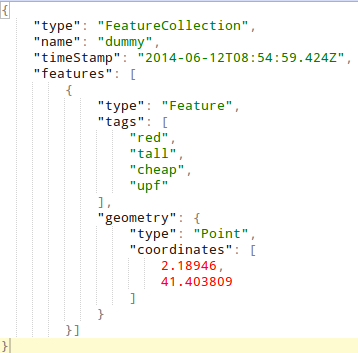
\includegraphics[scale=0.5]{./Figures/GeoJSON.png}
            \\
            \rule{15em}{0.5pt}
        \caption[GeoJSON message]{GeoJSON message.}
        \label{fig:GeoJSON}
      \end{figure}
    
  \section{Community network}
    Guifi\footnote{\url{https://www.guifi.net/}} is the network where the Arduino nodes will be deployed, and the one providing the access to Opencities through the Internet.
    Guifi is a network created by people interested in building an open, free and neutral network infrastructure.
    
    Because of their philosophy of participation, Guifi is the perfect network for the deployment of this sensor nodes. Also their network is large enough to become a useful sensor network (Figure \ref{fig:Guifimap}).
    \begin{figure}[htbp]
      \centering
          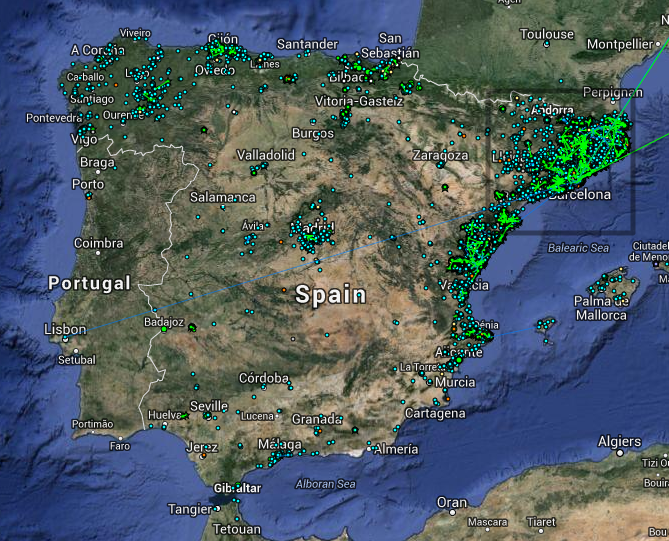
\includegraphics[scale=0.5]{./Figures/Guifimap.png}
          \rule{25em}{0.5pt}
      \caption[Guifi nodes]{Guifi nodes.}
      \label{fig:Guifimap}
    \end{figure}
    
  \section{Storage Resource Broker}  
    Opencities \cite{opencities} is the opendata service that has been chosen, for these reasons:
    \begin{itemize}
      \item The developers are at UPF, so the process of improving both projects (feedback, bug fixing, etc) can be fast and effective.
      \item Easy API to upload and download the data.
    \end{itemize}
    
    The role of Opencities is to be the intermediary between data creators and data users.
    In Opencities, the sensor data is uploaded to a dataset. Every user has an unique API key, and can create one or more datasets with a unique ID for each one. 
    
  \section{Visualization platform}
    
    For the purpose of the sensor data visualization there are several options, in plain text, in a map, in graphics, etc. In this project a map is used to display the data. This can be done on a web page, in a mobile application, tablet application, etc.
    
    Since the goal is that a user checks it for a small period of time, the best option is a mobile application. Additionally, almost everybody has a smartphone.
    
    There are three mobile operating system, iOS, Android, or Windows Phone. There is another option that is to developed the application in Html, Javascript, and CSS, and then compile it with Phonegap\footnote{\url{http://phonegap.com/}}, which builds the application for the three operating systems. This system ends up being much more difficult than to create an application directly to an operating system.
    Of the three operating systems, the one with more market share has been chosen to reach as many people as possible, so the Android operating system has been chosen.
      
    Android is a mobile operating system developed by Google, it runs on smartphones, and applications are programmed in Java. Java is a computer programming language that is object-oriented.    
    This application will be tested on a Sony Xperia Z1, with an Android 4.4.2.

\chapter{Bottom up sensor testbed}
\label{Chapter4}

  This chapter is focused on the process followed during the project, which has two main parts, the software to collect and send the data and the Android application to show it. A scheme of the project is shown in Figure \ref{fig:reportGeneralView}.
  
  \begin{figure}[htbp]
    \centering
        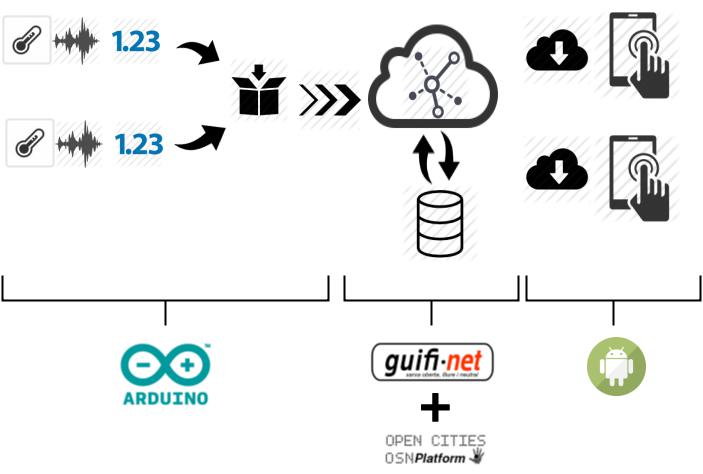
\includegraphics[scale=0.5]{./Figures/reportGeneralView.jpg}
        \rule{25em}{0.5pt}
    \caption[General View]{General View.}
    \label{fig:reportGeneralView}
  \end{figure}
  
  \section{Arduino Development}
    
    Two scripts are needed, one to collect the data, and other to send it. This is because the memory to run an Arduino sketch is very low, and the creation of the GeoJSON message is too big with respect to the available memory. That is why a Python script has been used, called first by the Arduino sketch.
    
    The Arduino sketch is responsible of collecting the data, write it in a logData file, and call the Python script with the collected values and an unique ID. Finally the Python script creates a GeoJSON message and sends it to Opencities.
    
    \subsection{Collect sensor data}
    
      To collect almost all the data the sketch does not need to include external libraries, except for the humidity sensors (DHT22 and DHT11)\footnote{\url{https://github.com/adafruit/DHT-sensor-library}}.
      
      The following libraries were needed to develop the code: FileIO, Process library, and Bridge.
      
      The Arduino sketch is coded in a very simple way, the setup function will initialize the Bridge library to communicate with the Linux environment, the Serial library for debugging purposes, and the FileSystem to log the process.
      The other function by default is the ``loop'', which calls three functions: readSensors, readFile, and executePythonScript.
      
      \begin{itemize}
        \item {\bf readSensors:} It calls 5 different functions to read every sensor, the reason for doing a separate function is to make the code more clear.
        \item {\bf readFile:} This function logs the process, saves the ID of the message, the sensor values, and a timestamp.
        \item {\bf executePythonScript:} The script in Python located in the SD card is in charge to create the GeoJSON message with all the sensor data and upload it to Opencities. This script is called by the Arduino sketch.
      \end{itemize}
      
      The Figure \ref{fig:Arduino sketch Flow Chart} explain how the Arduino sketch works.\\
      
      \begin{figure}[htbp]
      \centering

      \begin{tikzpicture}[node distance=2cm]

        \node (bridge) [startstop] {Initialize Bridge};
        \node (Serial) [process, below of=bridge] {Initialize Serial};
        \node (FileSystem) [process, below of=Serial] {Initialize FileSystem};
        \node (ReadSensors) [process, below of=FileSystem] {Read Sensors};
        \node (ReadFile) [process, below of=ReadSensors] {Read \& Write File};
        \node (delay) [process, right of=ReadFile, xshift=2cm] {Delay of 48 seconds};
        \node (ExecutePython) [process, below of=ReadFile] {Execute Python Script};
        
        \draw [arrow] (bridge) -- (Serial);
        \draw [arrow] (Serial) -- (FileSystem);
        \draw [arrow] (FileSystem) -- (ReadSensors);
        \draw [arrow] (ReadSensors) -- (ReadFile);
        \draw [arrow] (ReadFile) -- (ExecutePython);
        \draw [arrow] (ExecutePython) -| (delay);
        \draw [arrow] (delay) |- (ReadSensors);

      \end{tikzpicture}
      \rule{35em}{0.5pt}
      \caption[Arduino sketch Flow Chart]{Arduino sketch Flow Chart.}
      \label{fig:Arduino sketch Flow Chart}
      \end{figure}
    
    \subsection{Communication with Opencities}
    
      To communicate with Opencities it is necessary to create an account, and a dataset to store the sensor data. At the end, the user has an API key and a dataset ID, the required information to upload and download data. 
      
      The communication with Opencities is done by means of a Python script. This are the packages needed into the Linux environment of the Arduino: distribute, python-openssl, geojson, geopy, and httplib2.
      
      The Python script has three processes. First it stores all the sensor data collected by the Arduino sketch into a class. Then it creates a GeoJSON message with all the data, and all the parameters needed to upload it into Opencities. Finally uploads the GeoJSON message.
      
      With all these libraries the script can communicate with Opencities and store the sensor data collected by the Arduino. The Figure \ref{fig:Python Script Flow Chart} explains how the Python script works.\\
      
      \begin{figure}[!htbp]
      \centering

      \begin{tikzpicture}[node distance=2cm]      
        
        \node (start) [startstop] {Called by the Arduino};
        \node (CorrectUsage) [decision, below of=start, yshift=-2cm] {Is the usage correct};
        \node (collectdata) [process, below of=CorrectUsage, yshift=-2cm] {Store the arguments as sensor data};
        \node (ShowCorrectWay) [process, right of=CorrectUsage, xshift=4cm] {Show the correct usage};
        \node (StopUsage) [startstop, right of=ShowCorrectWay, xshift=2cm] {Stop};
        \node (CreateGeoJSON) [process, below of=collectdata] {Create GeoJSON};
        \node (PostOpencities) [process, below of=CreateGeoJSON] {POST in Opencities};
        \node (stop) [startstop, below of=PostOpencities] {Stop};
        
        \draw [arrow] (start) -- (CorrectUsage);
        \draw [arrow] (CorrectUsage) -- node[anchor=east] {yes} (collectdata);
        \draw [arrow] (CorrectUsage) -- node[anchor=south] {no} (ShowCorrectWay);
        \draw [arrow] (ShowCorrectWay) -- (StopUsage);
        \draw [arrow] (collectdata) -- (CreateGeoJSON);
        \draw [arrow] (CreateGeoJSON) -- (PostOpencities);
        \draw [arrow] (PostOpencities) -- (stop);
        

      \end{tikzpicture}
      \rule{35em}{0.5pt}
      \caption[Python Script Flow Chart]{Python Script Flow Chart.}
      \label{fig:Python Script Flow Chart}
      \end{figure}
      
  \section{Android app}
  
    \subsection{Summary}

      To easily visualize the results of the testbed, an Android application has been developed which shows the sensor data in a map. The application shows the data in two ways, with markers that show the actual value in that point, and also with heatmap points, the larger the value, the more intense the red will be (Figure \ref{fig:AppScreenshots}).
      
    \subsection{Interface}
      The application interface is a map view where the user can zoom, go to his location, and use the top buttons to change the sensor read. From left to right, the first button is the Marker button, the user decides whether the markers are displayed or not, and the next buttons refer to the type of sensor data to show as markers and/or as heatmap points (Temperature, Humidity, Noise, Light, and Air Quality).
      If the Marker button is checked, the user can click on the marker in the map and it will show the value and the unit of the temperature, humidity, noise, light, and air quality  (Figure \ref{fig:AppScreenshots}).
      \begin{figure}
        \centering
        \begin{subfigure}[b]{0.3\textwidth}
                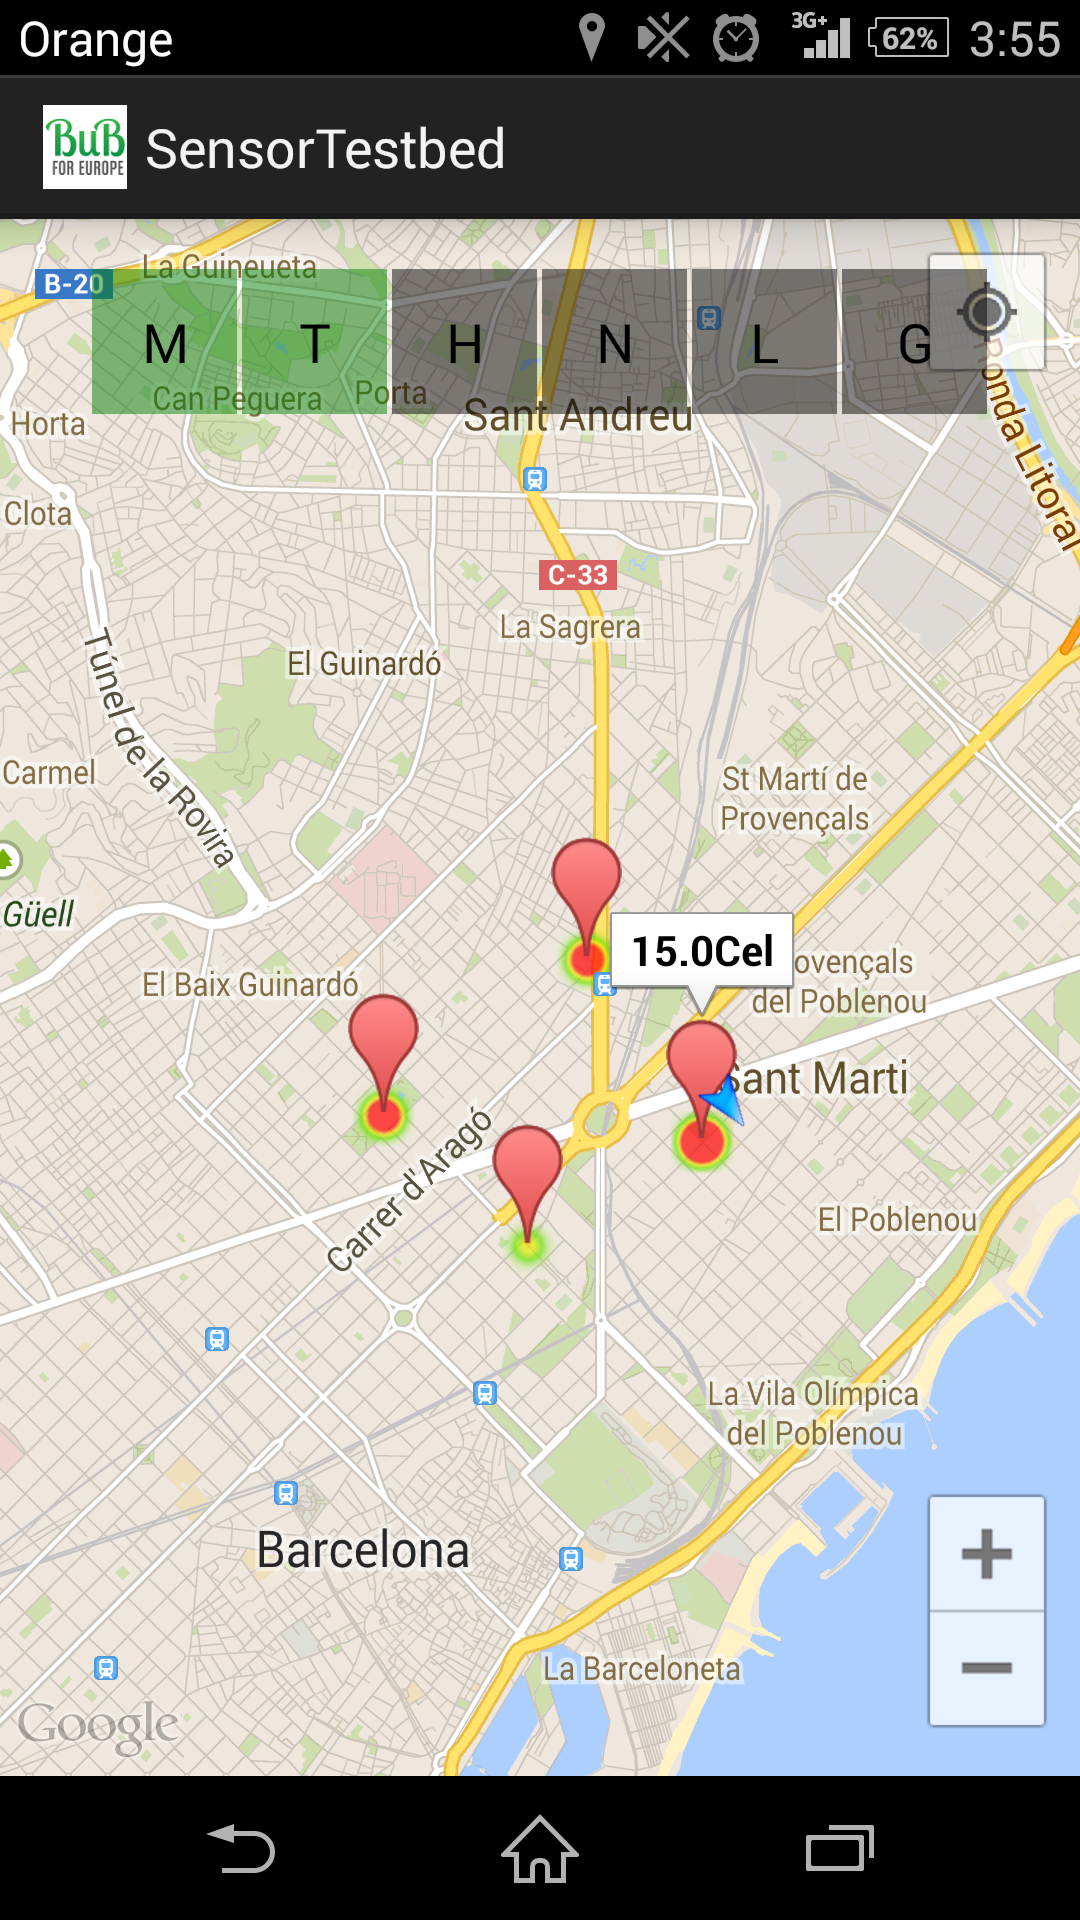
\includegraphics[width=\textwidth]{./Figures/App_Screenshot_1.png}
                \label{fig:App_Screenshot_1}
        \end{subfigure}%
        ~ %add desired spacing between images, e. g. ~, \quad, \qquad, \hfill etc.
          %(or a blank line to force the subfigure onto a new line)
        \begin{subfigure}[b]{0.3\textwidth}
                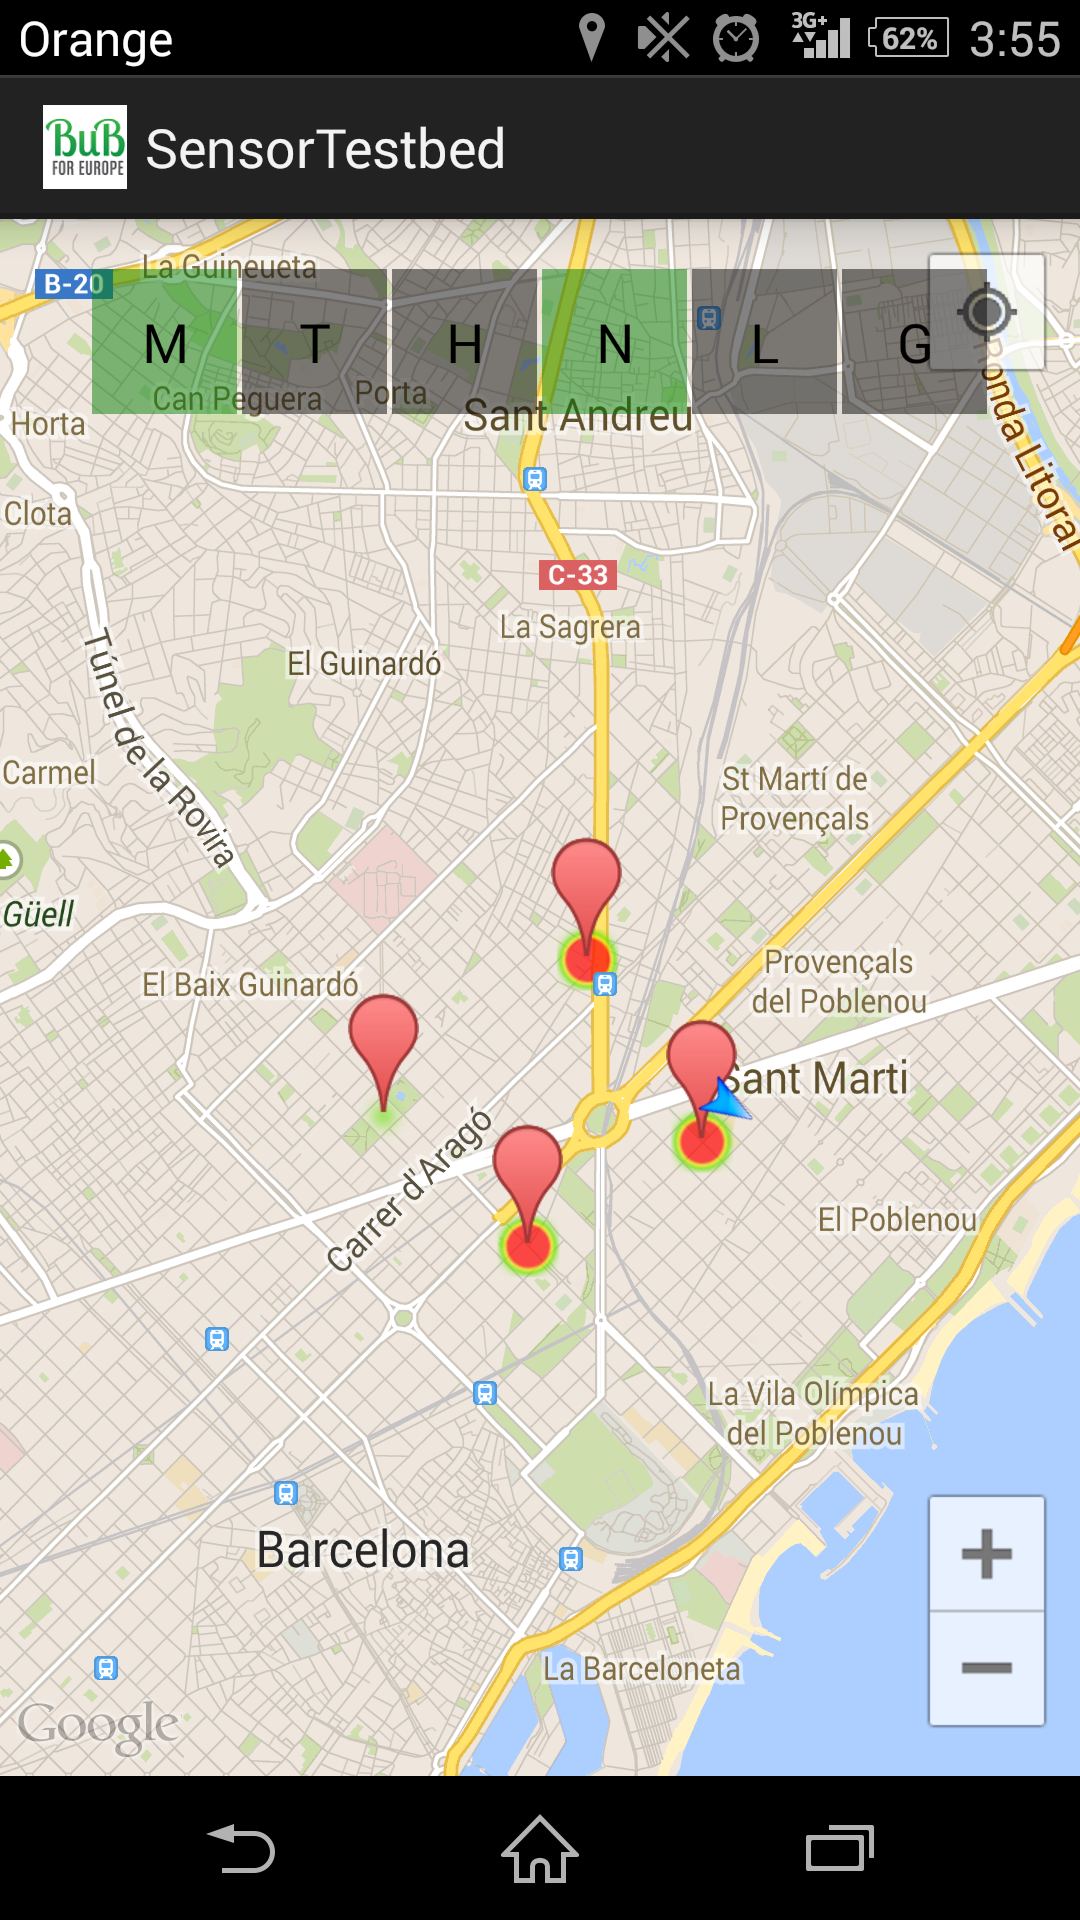
\includegraphics[width=\textwidth]{./Figures/App_Screenshot_3.png}
                \label{fig:App_Screenshot_2}
        \end{subfigure}
        \rule{18em}{0.5pt}
        \caption{App Screenshots}\label{fig:AppScreenshots}
\end{figure}
      
    \subsection{Code}
      First of all, to create this application the Google Maps Android API v2\footnote{\url{https://developers.google.com/maps/documentation/android/}} for the map view, and the Google Maps Android API utility library\footnote{\url{http://googlemaps.github.io/android-maps-utils/}} for the heatmaps have been used.
      
      In this application each class has a defined function, starting with MainActivity, which is the one that initialize the other classes, calls all the functions needed in the other classes to get the application started.
      It also has all the code to interact with the interface. For example, if the user clicks on the marker button, this class has to call all the necessary functions and display all the markers into the map.
      
      Next comes the dataBase class, which is the class that stores and processes the data downloaded from Opencities. This is a Singleton class, which means that there will only be one instance of this class and any instance of any class could access to the data stored in it.
      
      To store the data from Opencities, a set of classes have been created. These classes are equivalent to the GeoJSON message. At the end, the data is stored in features, which is composed primarily of Geometry and Properties.
      Then a class called HttpAsyncTask, that handles the communication with Opencities, stores the downloaded data using an instance of dataBase.
      
      Finally, a GPSTracker class is responsible for obtaining user location to place the map on the user location.
           
      The Figure \ref{fig:ClassDiagram} shows a simple class diagram where it only shows the class name and the connections between them.
      
      \begin{figure}[htbp]
        \centering
          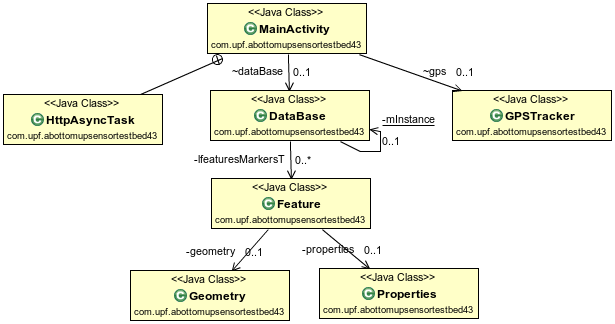
\includegraphics[page=1,scale=0.8]{./Figures/SmallClassDiagram.png}
        \rule{20em}{0.5pt}
        \caption[Simple Class Diagram of the Android App]{Simple Class Diagram of the Android App.}
        \label{fig:ClassDiagram}
      \end{figure}
      
      The explanation of the code is in the flow chart \ref{fig:Android App Flow Chart}.
      
      \begin{figure}[!htbp]
      \centering

      \begin{tikzpicture}[node distance=1cm]      
        
        \node (start) [startstop] {Initialize Google Map};
        \node (zoomlimit) [process, below of=start, yshift=-0.5cm] {Set zoom limit};
        \node (InitializeButtons) [process, below of=zoomlimit, yshift=-0.5cm] {Initialize all the Buttons and listeners};
        \node (GetCurrentLocation) [process, below of=InitializeButtons, yshift=-1cm] {Get Current Location using GPSTracker};
        \node (CallOpendata) [process, below of=GetCurrentLocation, yshift=-1cm] {Call OpenData, and parse the JSON};
        \node (CreateFeaturesByCoordinates) [process, below of=CallOpendata, yshift=-2cm] {Create a hashmap with all the features with the  coordinates as key, and a list of features for every key};
        \node (addMarkers) [process, below of=CreateFeaturesByCoordinates, yshift=-2cm] {Save only the latest features for every coordinate};
        \node (addHeatMapAndaddMakers2) [process, below of=addMarkers, yshift=-1.5cm] {Show the markers or heatmap points of a type of data};
        
        \draw [arrow] (start) -- (zoomlimit);
        \draw [arrow] (zoomlimit) -- (InitializeButtons);
        \draw [arrow] (InitializeButtons) -- (GetCurrentLocation);
        \draw [arrow] (GetCurrentLocation) -- (CallOpendata);
        \draw [arrow] (CallOpendata) -- (CreateFeaturesByCoordinates);
        \draw [arrow] (CreateFeaturesByCoordinates) -- (addMarkers);
        \draw [arrow] (addMarkers) -- (addHeatMapAndaddMakers2);
        

      \end{tikzpicture}
      \rule{35em}{0.5pt}
      \caption[Android App Flow Chart]{Android App Flow Chart.}
      \label{fig:Android App Flow Chart}
      \end{figure}

	\section{Repository}
		All the code, report, figures, etc has been stored in a public repository\footnote{\url{https://github.com/SergioAlmendros/A-bottom-up-sensor-testbed}}, so anyone could see it, download a copy, and change it if necessary.
		
		The Figure \ref{fig:repository} illustrates how the repository is organized, each folder represents part of the process that has been done in this project.
		
		\begin{figure}[htbp]
			\centering
				  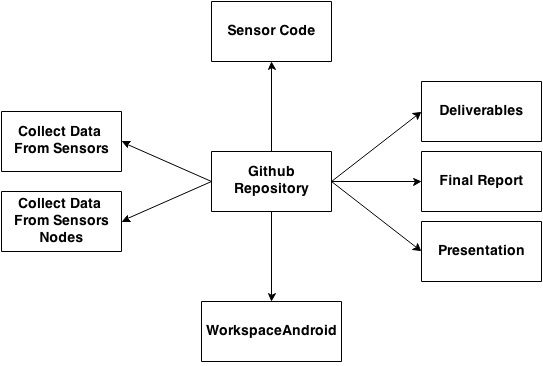
\includegraphics[scale=0.6]{./Figures/repository.png}
				  \rule{25em}{0.5pt}
			\caption[Github Repository]{Github Repository.}
			\label{fig:repository}
		\end{figure} 
		
		The most important folders are:
		\begin{itemize}
			\item {\bf Sensor Code:} Where the code has been stored that runs into the Arduino (Arduino sketch and Python script).
			\item {\bf WorkspaceAndroid:} This folder has been used as workspace for the developing of the mobile application using the Eclipse IDE (Integrated Development Environment).
			\item {\bf Final Report:} Is where the project it has been documented. The report has been written in Latex, a system for the presentation of technical and scientific documentation.
		\end{itemize}
		
		The other folders are:
		\begin{itemize}
			\item {\bf Collect Data From Sensors:} Here it has been stored the code to get the value of each sensor separately, for easier reusability of the code.
			\item {\bf Collect Data From Sensors Nodes:} Using the logData files that have been created during the testbed, an octave script reads this data and displays it through graphs.
			\item {\bf Deliverables:} In this folder the initial documentation of the project has been stored, that are reported in the Appendices \ref{PilotCharter} and \ref{PlanningReport}.
			\item {\bf Presentation:} Finally, here is the slide presentation that has been made to explain the project.
		\end{itemize}
		
		During all the project there have been constant uploads of new information to the repository, as it was evolving.


\chapter{Testbed Deployment and Results}
\label{Chapter5}

  This chapter explains the procedure to deploy a testbed step by step.
  
  In the Figure \ref{fig:TestBed_Prototype} there is a photograph of the prototype used in this testbed. It is composed of an Arduino YUN,- a microSD card, a breadboard, and all the sensor connected (temperature, humidity, noise, light, and gas) to the Arduino YUN.
  
  \begin{figure}[htbp]
      \centering
          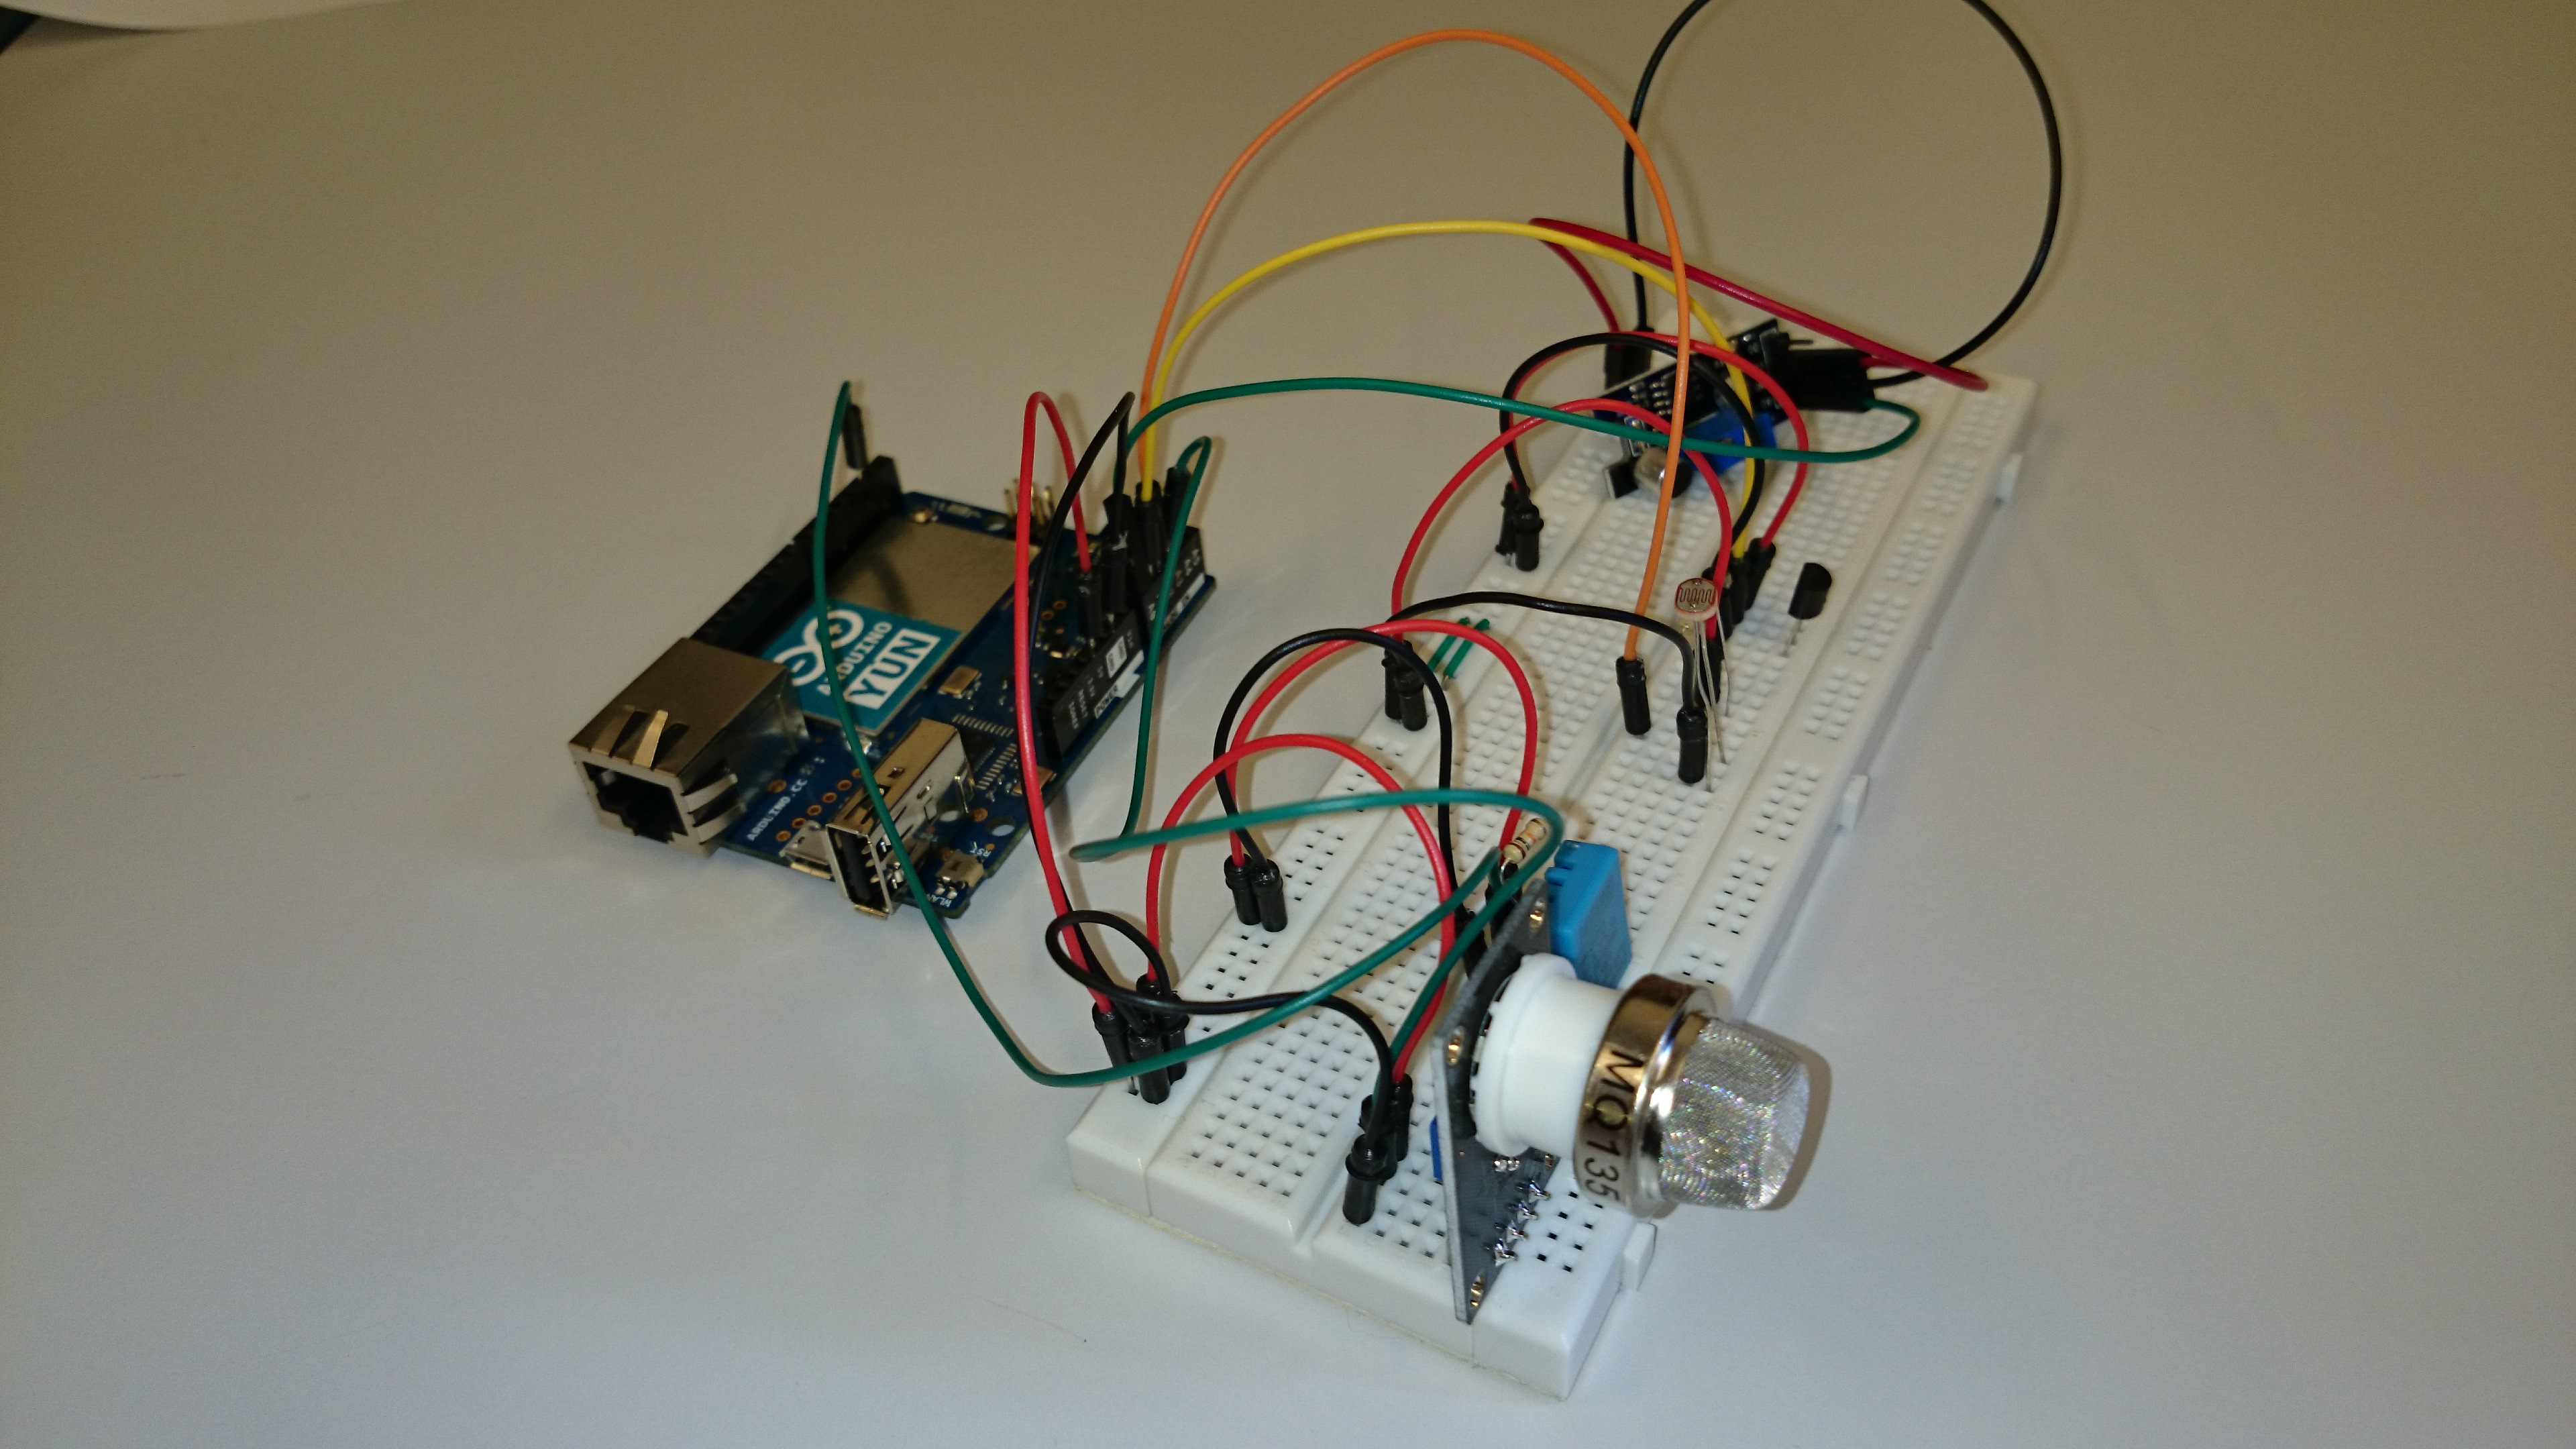
\includegraphics[scale=0.1]{./Figures/prototype.png}
          \rule{35em}{0.5pt}
      \caption[TestBed Prototype]{TestBed Prototype.}
      \label{fig:TestBed_Prototype}
  \end{figure} 
  
  \section{Sensor node}
  
  	This section shows the process to configure the sensor node \cite{guideArduinoYun}:
  
  \subsection{Connection to the Internet}
    First of all an Internet connection has to be provided to the Arduino.
    \subsubsection{Through Ethernet}
      This is the fastest way to provide Internet connection, the Arduino automatically obtains an IP address.
      
    \subsubsection{Through WiFi}
      This is the slowest way. The process is the following:
      \begin{enumerate}
        \item After powering the Arduino YUN, it creates his own WiFi network (ArduinoYun-XXXXXXXXXXXX).
        \item After connecting to the YUN network, the address \url{http://arduino.local} or \url{192.168.240.1} can be accessed and the password should be provided. The default password is ``arduino''. The procedure is shown in the Figure \ref{fig:YunWebPassword}.
          \begin{figure}[htbp]
            \centering
                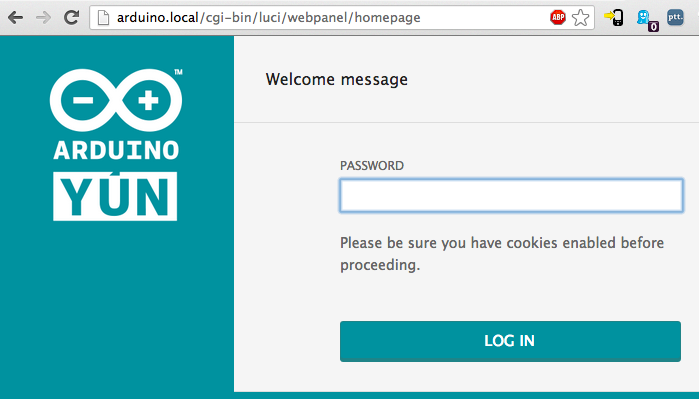
\includegraphics[scale=0.3]{./Figures/YunWebPassword.png}
                \rule{18em}{0.5pt}
            \caption[Yun web Password]{Yun web Password.}
            \label{fig:YunWebPassword}
          \end{figure}
        
        \item After providing the password, an information page is displayed, as shown in Figure \ref{fig:YunWebDiagnostic}.
          \begin{figure}[htbp]
            \centering
                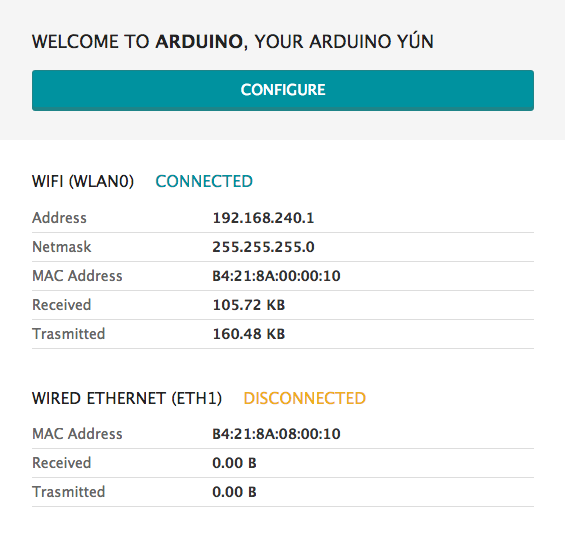
\includegraphics[scale=0.3]{./Figures/YunWebDiagnostic.png}
                \\
                \rule{15em}{0.5pt}
            \caption[Yun web Diagnostic]{Yun web Diagnostic.}
            \label{fig:YunWebDiagnostic}
          \end{figure}
        
        \item It is necessary to tell the Yun what network to connect to, and after pressing the the configure \& restart button, the computer can connect to the Yun through the wifi network (Figure \ref{fig:YunWebConfig}).
          \begin{figure}[htbp]
            \centering
                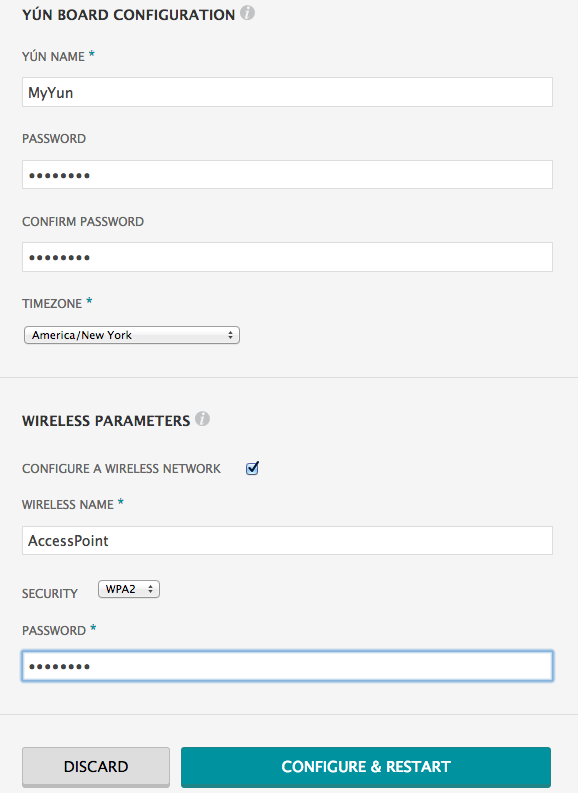
\includegraphics[scale=0.3]{./Figures/YunWebConfig.png}
                \\
                \rule{15em}{0.5pt}
            \caption[Yun web Configuration]{Yun web Configuration.}
            \label{fig:YunWebConfig}
          \end{figure}
        
      \end{enumerate}
  \subsection{Install necessary packets}
    The Arduino runs an Arduino sketch and a Python script, for the Python script some packets have to be installed.
    
    To install any packet, a ssh connection to the arduino has to be created (as shown before):
    
    {\begin{centering} \textbf{ssh root@X.Y.Z.W}\par \end{centering}}
    
    The required commands are the following:
     
      {\begin{centering} \textbf{
          opkg update \\
          opkg install distribute \\
          opkg install python-openssl \\
          easy\_install install geojson \\
          easy\_install install geopy \\
          easy\_install install httplib2
        }
      \par \end{centering}}
    
  \subsection{Copy the scripts}
    First of all, it is necessary to create some directories, the following commands have to be executed:
    
    {\begin{centering} \textbf{
    cd /mnt/sda1 \\
    mkdir arduino \\
    cd arduino \\
    mkdir www \\
    }\par \end{centering}}
    
    After connecting to the YUN network, the address http://arduino.local can be accessed and the password should be provided. The default password is “arduino”. The procedure is shown in the Figure 5.2.
    
    After these processes have finished, the Python script ``main.py'' should be copied into the SD-Card. There are two ways to do this, putting the SDCard into a computer an saving the file directly, or copying the file into the Arduino through the network with the following command:
    
    {\begin{centering} \textbf{
    scp main.py root@192.168.2.149:/mnt/sda1/arduino/www/main.py
    }\par \end{centering}}
  
  \subsection{Attach the sensors}
    Now that the Python step is done, the sensors have to be attached to the Arduino Yun (Figure \ref{fig:AllSensors22_bb} or Figure \ref{fig:AllSensors11_bb}).
  
  \subsection{Arduino Code}
    To upload an Arduino sketch to the Yun the IDE (Arduino 1.5.5) has to be used. There are two ways to upload a sketch, through an USB cable connected to the Arduino, or through the Internet. If the Arduino and the computer are in the same network, the Arduino will appear in the IDE as a possible device to connect with.
  
  \section{Actual Testbed}
    Three Arduino nodes were built and placed in three different locations.
    
    The unique ID has to be introduced manually into the Arduino sketch with the Arduino IDE and the location into the Python script by logging into the Arduino by secure shell and modifying the following line in ``main.py'':
    
    {\begin{centering} \textbf{self.address = 'Sagrada Familia, Carrer de Mallorca, Barcelona'}\par \end{centering}}
    
    After a day of collecting data, the three logData files has been analyzed, and some graphs to show the data had been made.
    
    The Figure \ref{fig:Testbedmap} shows the nodes deployed.
    \begin{figure}[htbp]
      \centering
          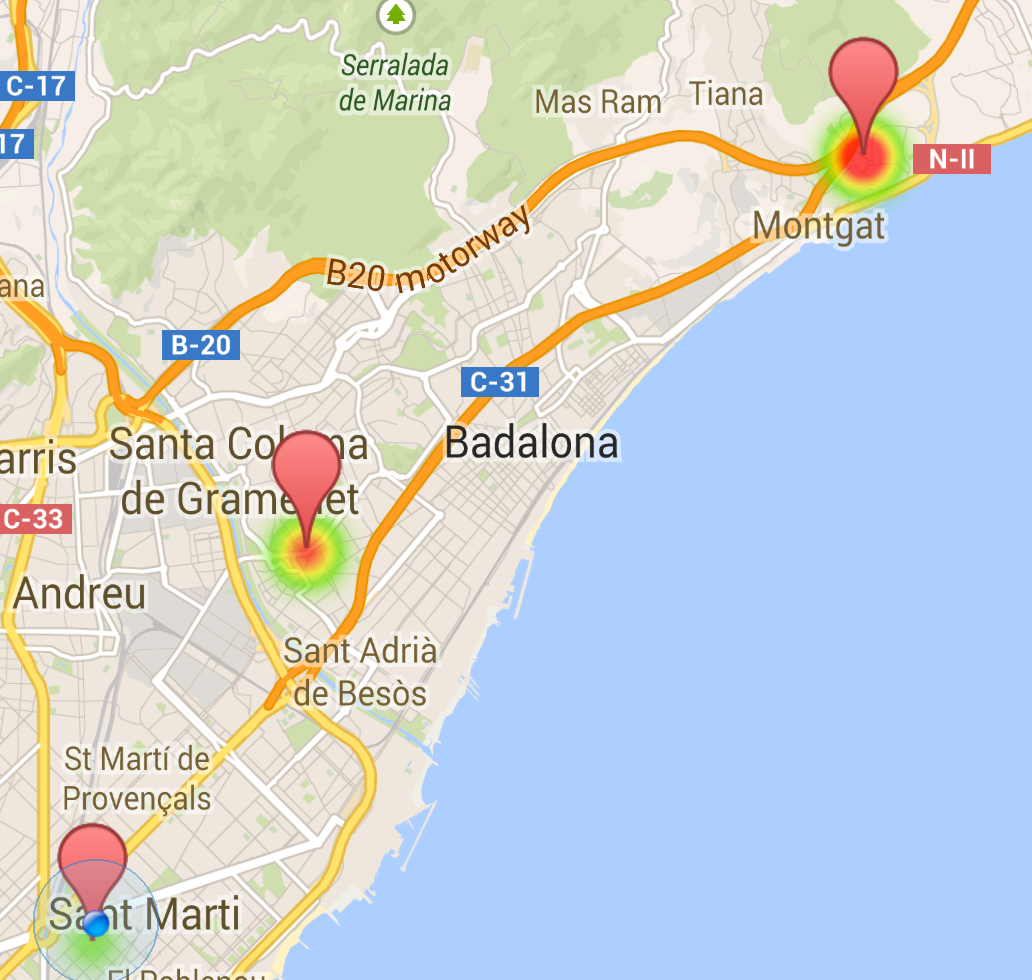
\includegraphics[scale=0.2]{./Figures/Testbedmap.png}
          \\
          \rule{15em}{0.5pt}
      \caption[Testbed Map]{Testbed Map.}
      \label{fig:Testbedmap}
    \end{figure}
    
    \subsection{Results}
      
      Thanks to the testbed a sensor network has been deployed, with three nodes, for economical reasons, without any problems.    
      
      A mobile application has been made, and shows an example that could led to more people to create other applications that work with the sensor data stored in Opencities. 
      The data has been stored on a platform and the mobile application has been able to access them. A problem happened, the application was not designed to cope with big amount of data, so it needs improvement.

      All the data produced during this testbed has been stored in the SD card of the Arduino nodes, and graphically displayed in figures: \ref{fig:GraphicTemperature}, \ref{fig:GraphicLight}, \ref{fig:GraphicNoise}, \ref{fig:GraphicHumidity}, \ref{fig:GraphicGas}.

      \begin{figure}[H]
        \centering
        \begin{subfigure}[b]{0.49\textwidth}
                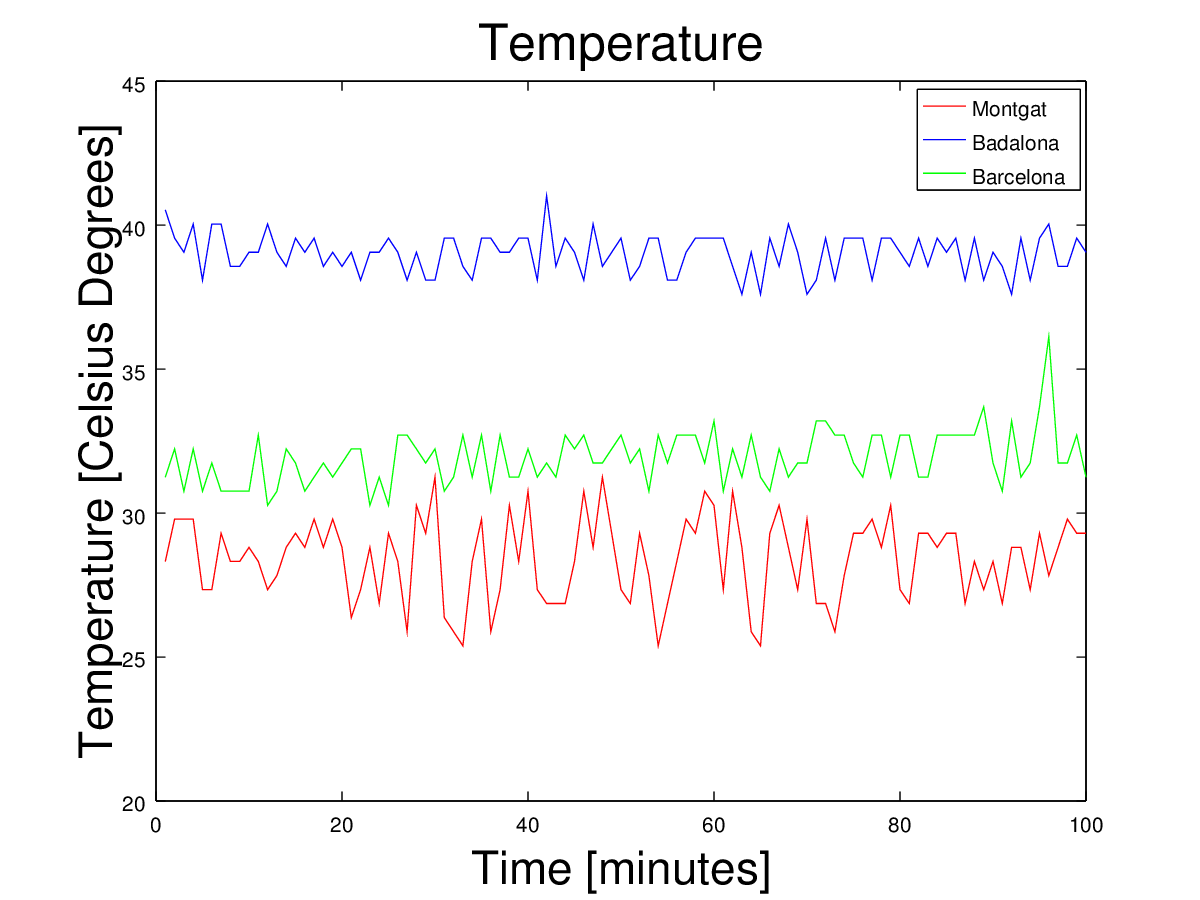
\includegraphics[width=\textwidth]{./Figures/GraphicTemperature.png}
                \caption{Graphic Temperature}
                \label{fig:GraphicTemperature}
        \end{subfigure}%
        ~ %add desired spacing between images, e. g. ~, \quad, \qquad, \hfill etc.
          %(or a blank line to force the subfigure onto a new line)
        \begin{subfigure}[b]{0.49\textwidth}
                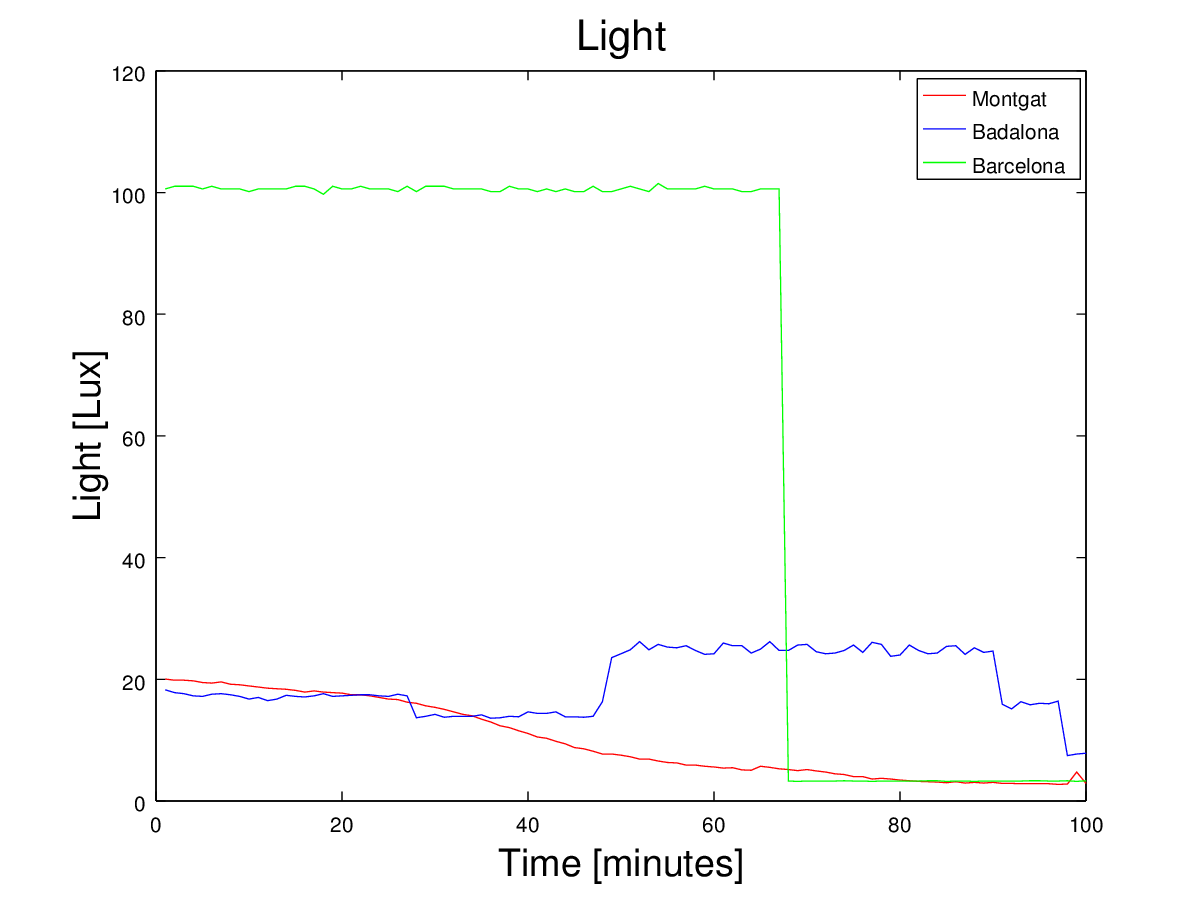
\includegraphics[width=\textwidth]{./Figures/GraphicLight.png}
                \caption{Graphic Light}
                \label{fig:GraphicLight}
        \end{subfigure}
        \rule{30em}{0.5pt}
        \caption{Temperature and Light Graphics, for 100 minutes acquisition window}\label{fig:TestbedResults1}
			\end{figure}
			\begin{figure}[H]
        \centering
        \begin{subfigure}[b]{0.49\textwidth}
                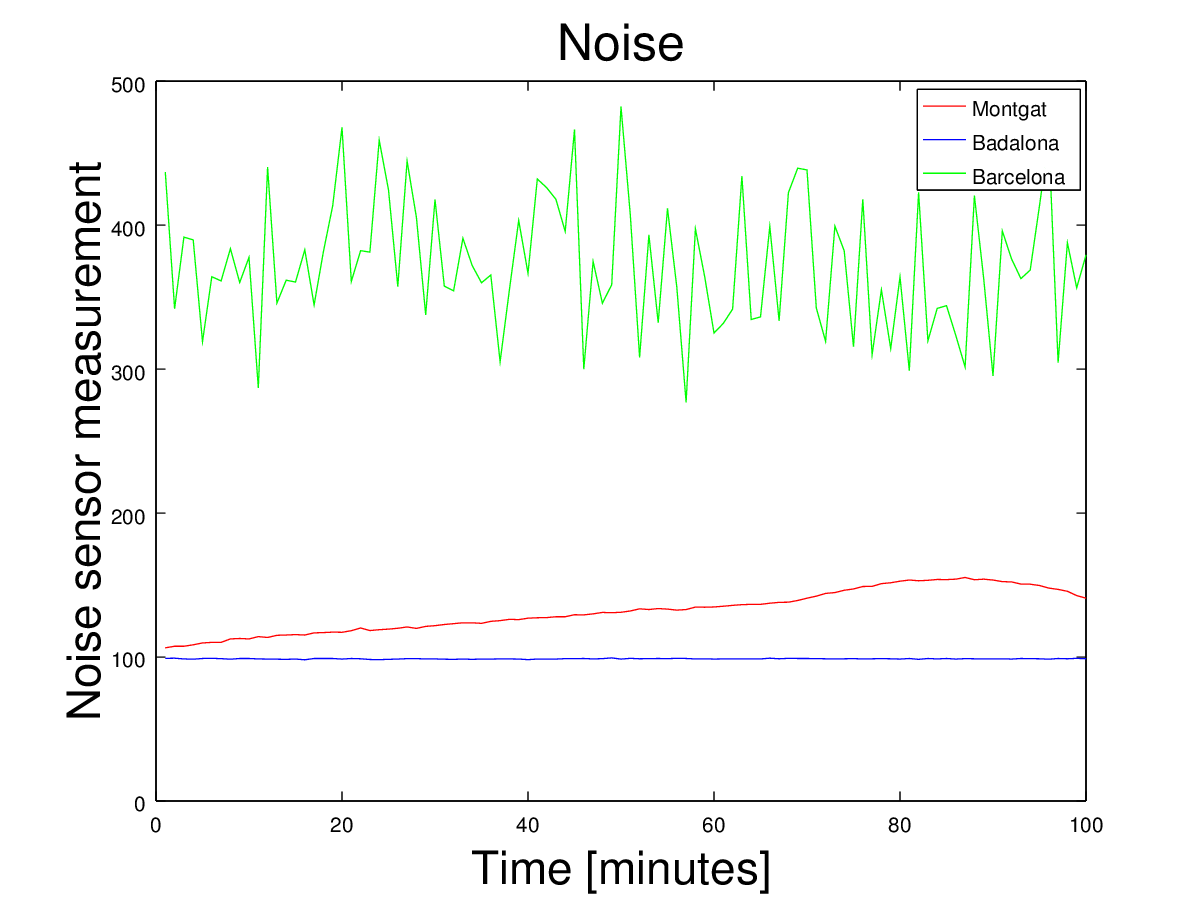
\includegraphics[width=\textwidth]{./Figures/GraphicNoise.png}
                \caption{Graphic Noise}
                \label{fig:GraphicNoise}
        \end{subfigure}%
        ~ %add desired spacing between images, e. g. ~, \quad, \qquad, \hfill etc.
          %(or a blank line to force the subfigure onto a new line)
        \begin{subfigure}[b]{0.49\textwidth}
                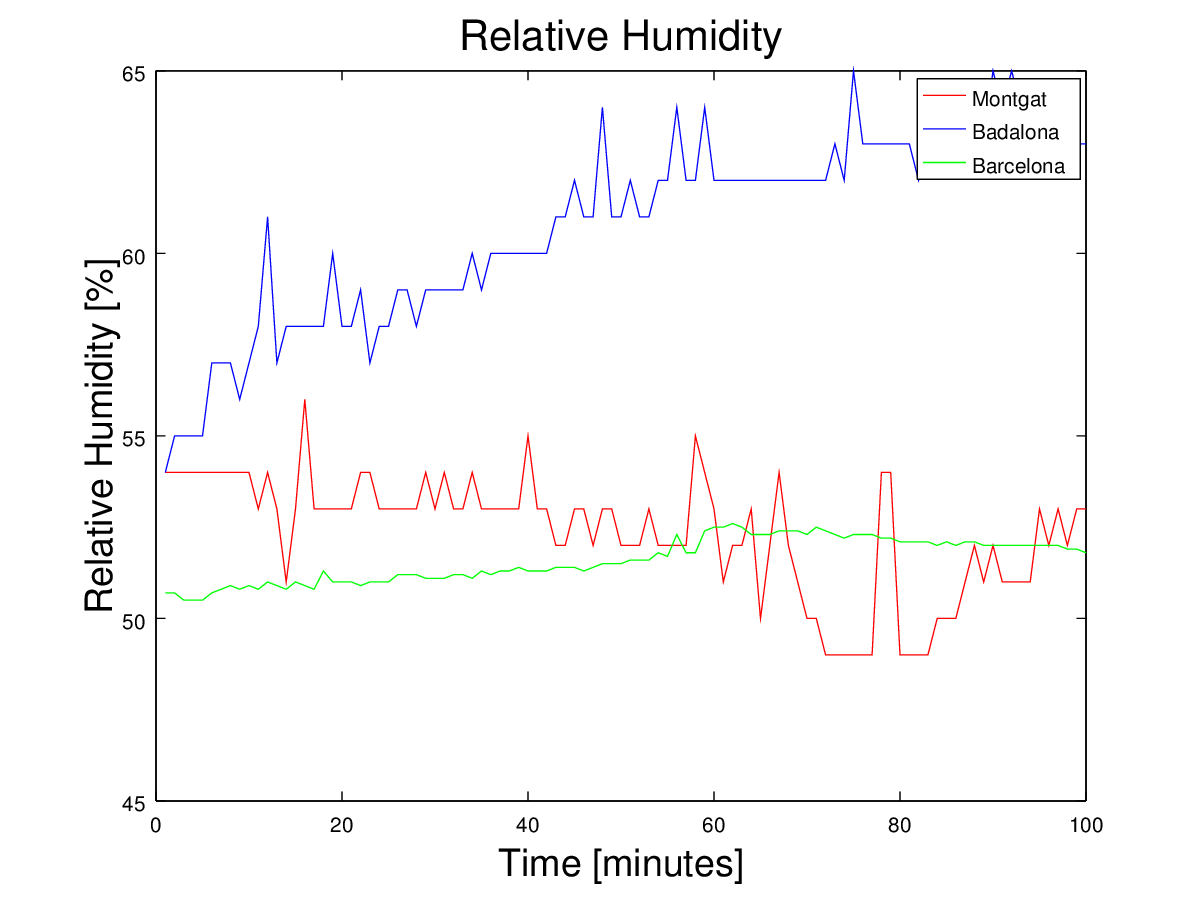
\includegraphics[width=\textwidth]{./Figures/GraphicHumidity.png}
                \caption{Graphic Humidity}
                \label{fig:GraphicHumidity}
        \end{subfigure}
        \rule{30em}{0.5pt}
        \caption{Noise and Humidity Graphics, for 100 minutes acquisition window}\label{fig:TestbedResults1}
			\end{figure}
			\begin{figure}[H]
		    \centering
		        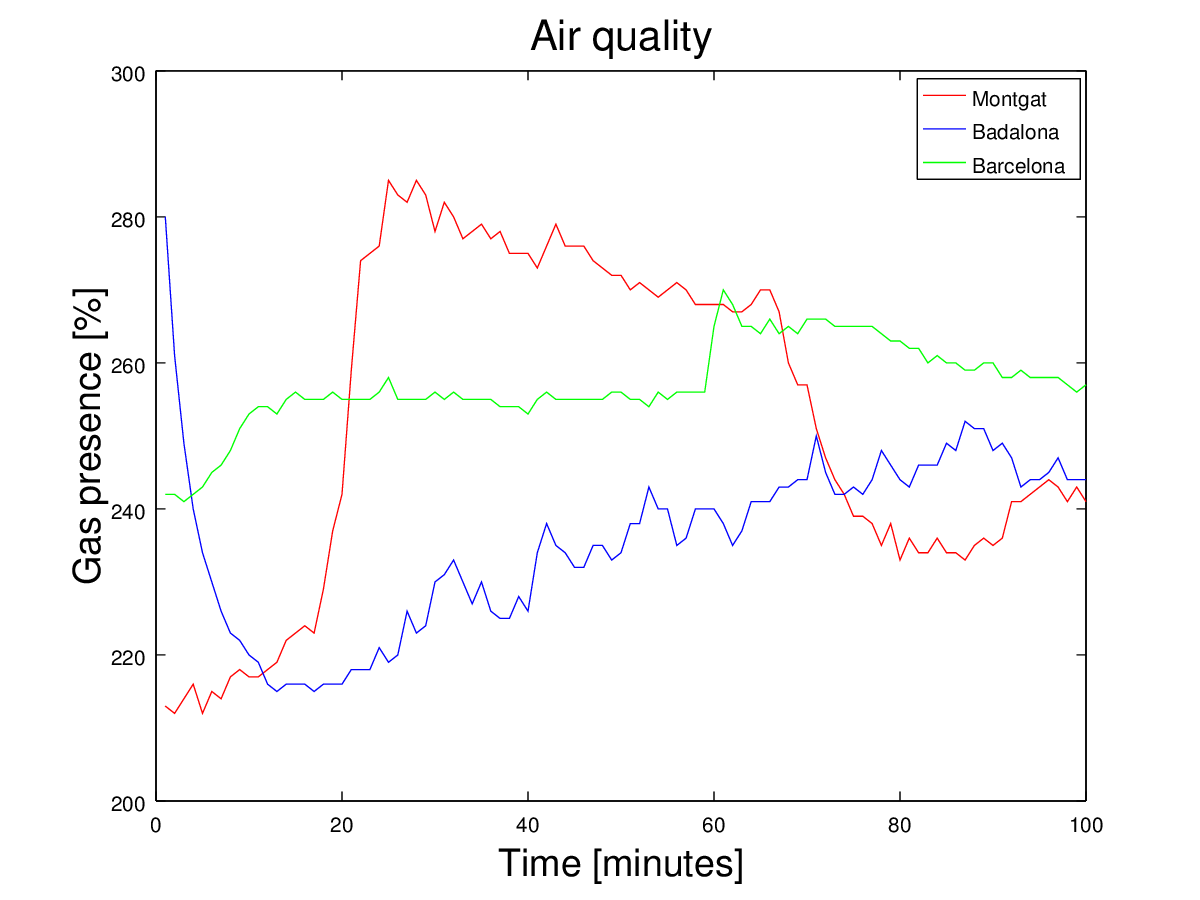
\includegraphics[scale=0.4]{./Figures/GraphicGas.png}
		        \rule{18em}{0.5pt}
		        \caption[Graphic Air Quality, for 100 minutes acquisition window]{Graphic Air Quality, for 100 minutes acquisition window.}
		        \label{fig:GraphicGas}
		  \end{figure}
			
			From the acquired data it is possible to draw some conclusions:
      
      The temperature is clearly higher in Badalona, but the three locations are not far apart, so this value should not vary much. It is important to notice that this is a low quality sensor so it is possible that it may have failed during the testbed since the graphs of Montgat and Barcelona are similar between them, but very different in comparison to Badalona.
      
      In the case of light, the sensor node in Barcelona receives direct sunlight during most of the day, but the node in Montgat and Badalona does not. Consequently, it is normal that the Barcelona node had a much higher light value.
      
      The Barcelona node collects noise values much higher than the other two nodes. The Badalona and Montgat nodes are in areas with punctual car traffic, while the Barcelona node is in a busy area, causing more noise.
      
      In the case of the relative humidity, the Badalona node is near a river and the Montgat node is near the sea, so it is logical that the Barcelona node measures less relative humidity.
      
      The Badalona node captures better air quality than the Barcelona and Montgat nodes. The Barcelona node collects constant values, more or less, which is normal because there is in an area with high car traffic. The Badalona node collects a decrease in air quality as time passes, which coincides with the arrival of workers who park in the area. In the case of Montgat, there is a big difference in a time slot. This node is located near a highway, so it is possible that this time slot coincide when there is more traffic on the highway.

\chapter{Conclusions}
\label{Chapter6}
  
  The deployment of a sensor network made during this project has been successful, this has proved that the sensor nodes have functioned properly.  
  Therefore, it has been shown that anyone can deploy its own network in an inexpensive way, with open source hardware and software, and easy to use.
  
  A mobile application has been developed to serve as an example, so the citizens who want to create their own mobile application find the process easier.
 	All the code that has been created during this project is open source and is available online, in a Github repository.
  
  In conclusion, the project had satisfied the goals presented in the project proposal, sharing sensor data on an open network, and giving the users the tools to visualize it.

\chapter{Future work}
\label{Chapter7}
  
  This project can be improved in two ways, the sensor node and the Android application.
  
  The sensor node could be ameliorated building a more compact and solid prototype, removing the breadboard. This prototype should be built bearing in mind that the node will be mounted outdoor. To be fully compatible with Guifi network, this prototype should be powered using PoE technology.
  
  The Android application showed some issues when requested to handle a lot of data. This issue can be solved downloading a limited set of data (e.g. the most recent).
  Moreover, the application can be improved adding the possibility to draw the history data.
  
  Finally the project could be disseminated by a web page or conference on sensors.

\bibliography{bibliography}
\phantomsection
\addcontentsline{toc}{chapter}{BIBLIOGRAPHY}
\cleardoublepage

\appendix
\label{Appendixes}

	\chapter{Pilot Charter}
	\label{PilotCharter}
  	\section{Pilot Charter}
\label{sec:mnp}

Fellow: Sergio Almendros Diaz
\\
Mentor: 
\\
Advisor: Jaume Barcelo

\subsection{Pilot purpose or justification}
The purpose of this pilot is to build a sensor platform that can be attached to guifi nodes to gather and share sensory data.

\subsection{Measurable pilot objectives and related success criteria}
\begin{itemize}
\item Gather data about temperature, humidity, light, and noise. 
\item Share the data as open data.
\item Deploy at least two nodes and gather data for at least two weeks.
\end{itemize}

\subsection{High-level requirements}
\begin{itemize}
\item Outdoor enclosure.
\item Use open hardware and open software to the possible extent.
\item Use standardized interfaces to integrate with other projects.
\end{itemize}

\subsection{High-level pilot description}
The goal is to use an arduino platform to create a bottom-up broadband wireless sensor networks. 
As guifi.net has already over 20,000 nodes, the idea is to co-locate the sensory platforms together with the guifi.net nodes and use the guifi.net network to transmit the data.
This data should be gathered and shared.
Ideally, the pilot should include a presentation interface for the users to visualize the data.

\subsection{High-level risks}
A possible risk is that the prototypes are not rugged enough for outdoor environments.
It is also a risk that the prototype is not stable and needs to be reset very often.

\subsection{Summary milestone schedule}
\begin{itemize}
\item From 20/09/2013 to 23/09/2013
	\begin{itemize}
	\item Establish the general idea of the TFG and specifics goals.
	\end{itemize}
\item From 23/09/2013 to 11/10/2013
	\begin{itemize}
	\item Specify the tasks to do and make a planning.
	\end{itemize}
\item From 11/10/2013 to 30/10/2013
	\begin{itemize}
	\item Connect first sensors to the Arduino.
	\end{itemize}
\item From 31/10/2013 to 10/01/2014
	\begin{itemize}
	\item Connect to guifi network and upload data to an open data platform.
	\end{itemize}
\item From 10/01/2014 to 01/06/2014
	\begin{itemize}
	\item Integration of sensors and communication aspects.
	\item Install prototypes.
	\item Data sharing and visualization.
    \item Data analysis and evaluation of the testbed.
	\end{itemize}
\item From 02/06/2014 to 30/06/20014
	\begin{itemize}
	\item Preparation of the final memory.
	\end{itemize}
\item From 01/07/2014 to the date of the presentation
	\begin{itemize}
	\item Make the presentation.
	\end{itemize}
\end{itemize}

\subsection{Summary budget}
The cost of this pilot will be approximately 4000 \euro. This quantity is for the scholarship to the student that will develop this pilot, budget for attending a conference or visiting collaborators, and the purchase of the necessary hardware.

	
	\chapter{Planning Report}
	\label{PlanningReport}
  	\documentclass[10pt,a4paper]{article}
\usepackage{pgfgantt}

\title{A bottom up sensor testbed}
\author{Sergio Almendros Diaz}
\date{\today}

\begin{document}
\maketitle

\section{Planning Report}

The following sections explain the tasks that I will do in the course of this project.

\subsection{Familiarization with the Arduino Yun}

In this project I will be working with an arduino Yun, but I never worked before with any type of arduino, so the first task is to start coding different kind of programs. Then I will have to learn how to interact with the linux in the arduino Yun.

\subsection{Small problem solution}

I want to do an easy example to how to connect an arduino with a server running in my computer, what I want to do is establish a bridge between an arduino program and the linux within the arduino to be able to communicate with a server in my laptop, and send a string with the value returned by a sensor.
This is a reduce problem of the real "bottom-up sensor testbed" because, at the end, in every arduino will be a program that will have to send a message to a server with the data of the sensors attached to it.

\subsection{Collect Data from sensors}

First I will connect a temperature sensor to the arduino YUN, then, I will develop a program to collect the information from it, and send it to a server.
When the temperature sensor works, I will do the same process with a humidity, light, and noise sensor.

\subsection{Install Sentilo}

Sentilo (www.sentilo.io) is an open source sensor and actuator platform that I will install in my laptop to act as the server between the sensor network and the interface for the users to visualize the data. 

\subsection{Communication with Sentilo}

I will adapt the messages that the arduino send to fit with the Sentilo.

\subsection{Real deployment}

At this moment, the part of the arduino and the server will be done, so I will test the server installing the arduino in real nodes of the guifi network, for example, the node in the Universitat Pompeu Fabra, and any other node that allow me to install it. The arduino will have a temperature, humidity, light, and noise sensor.

\subsection{Interface}

I want to do an interface for any user to understand the meaning of the temperature, humidity, light, and noise values. This interface will be develop for an android mobile application.

\subsection{Sentilo module}

I will contribute to Sentilo and other sensor data brokerage platforms accommodating the sensor testbed deployed in the previous tasks.

\subsection{Final report}

This task have to be done in parallel with all the other ones, and its purpose is document all the work that I will do.

\subsection{Gantt chart}

\begin{figure}
\begin{center}
  \begin{ganttchart}{1}{23}
    \gantttitle{Pilot Timeline}{23} \\ 
    \ganttbar{Task 1 [7/01/14 - 12/01/14]}{1}{1} \\
    \ganttlinkedbar{Task 2 [13/01/14 - 19/01/14]}{3}{4} \\
    \ganttlinkedbar{Task 3 [20/01/14 - 2/02/14]}{5}{7} \\
    \ganttlinkedbar{Task 4 [3/02/14 - 5/02/14]}{8}{8} \\
    \ganttlinkedbar{Task 5 [6/02/14 - 16/02/14]}{9}{11} \\
    \ganttlinkedbar{Task 6 [17/02/14 - 2/03/14]}{12}{13} \\
    \ganttlinkedbar{Task 7 [3/03/14 - 30/04/14]}{14}{18} \\
    \ganttlinkedbar{Task 8 [1/05/14 - 31/06/14]}{19}{22} \\
    \ganttbar{Task 9 [7/01/14 - 31/06/14]}{1}{22}
  \end{ganttchart}
\end{center}
\end{figure} 
 

\end{document}

  	
  \chapter{Class Diagram}
	\clearpage
		\begin{figure}[H]
      \centering
        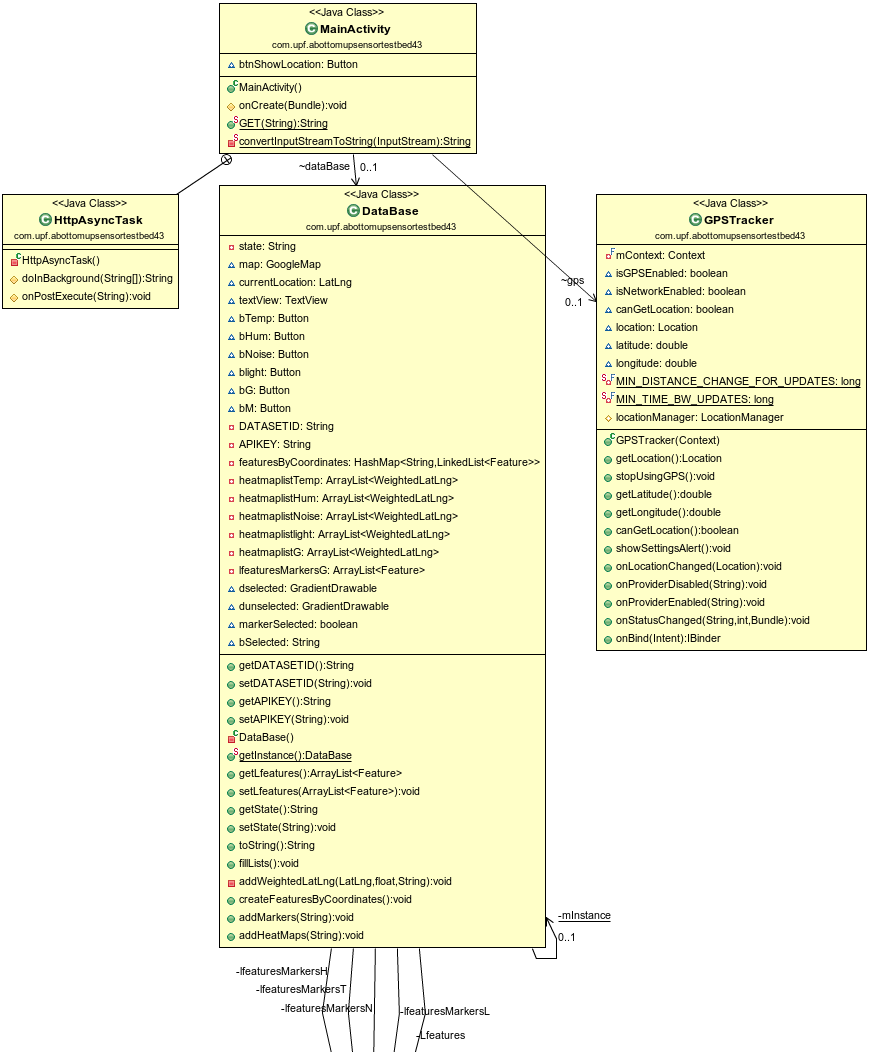
\includegraphics[scale=0.5]{./Figures/ClassDiagram1_1.png}
      \rule{35em}{0.5pt}
      \caption[Class Diagram of the Android App part 1]{Class Diagram of the Android App part 1.}
      \label{fig:ClassDiagram1}
    \end{figure}
		
    \begin{figure}[H]
      \centering
        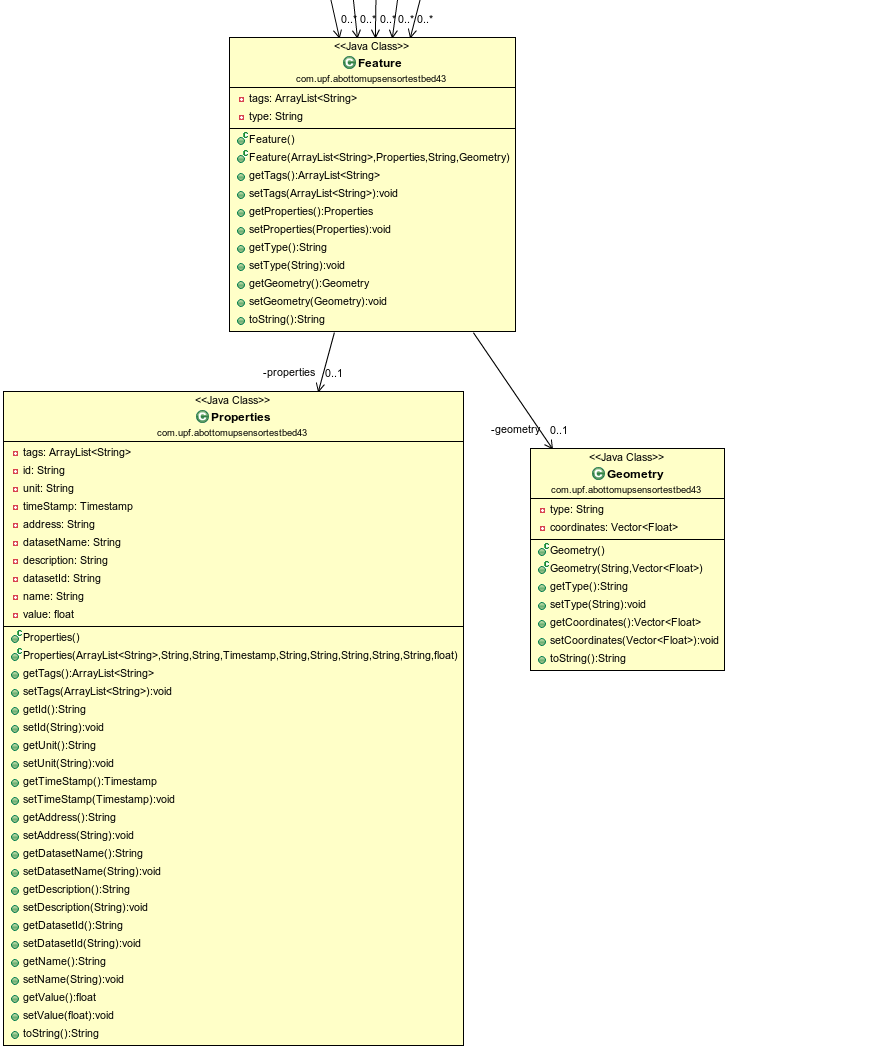
\includegraphics[scale=0.5]{./Figures/ClassDiagram1_2.png}
      \rule{35em}{0.5pt}
      \caption[Class Diagram of the Android App part 2]{Class Diagram of the Android App part 2.}
      \label{fig:ClassDiagram2}
    \end{figure}
  
  \chapter{Testbed Graphics}
  \label{testbedgraphicsappendix}
  	\begin{figure}[H]
      \centering
        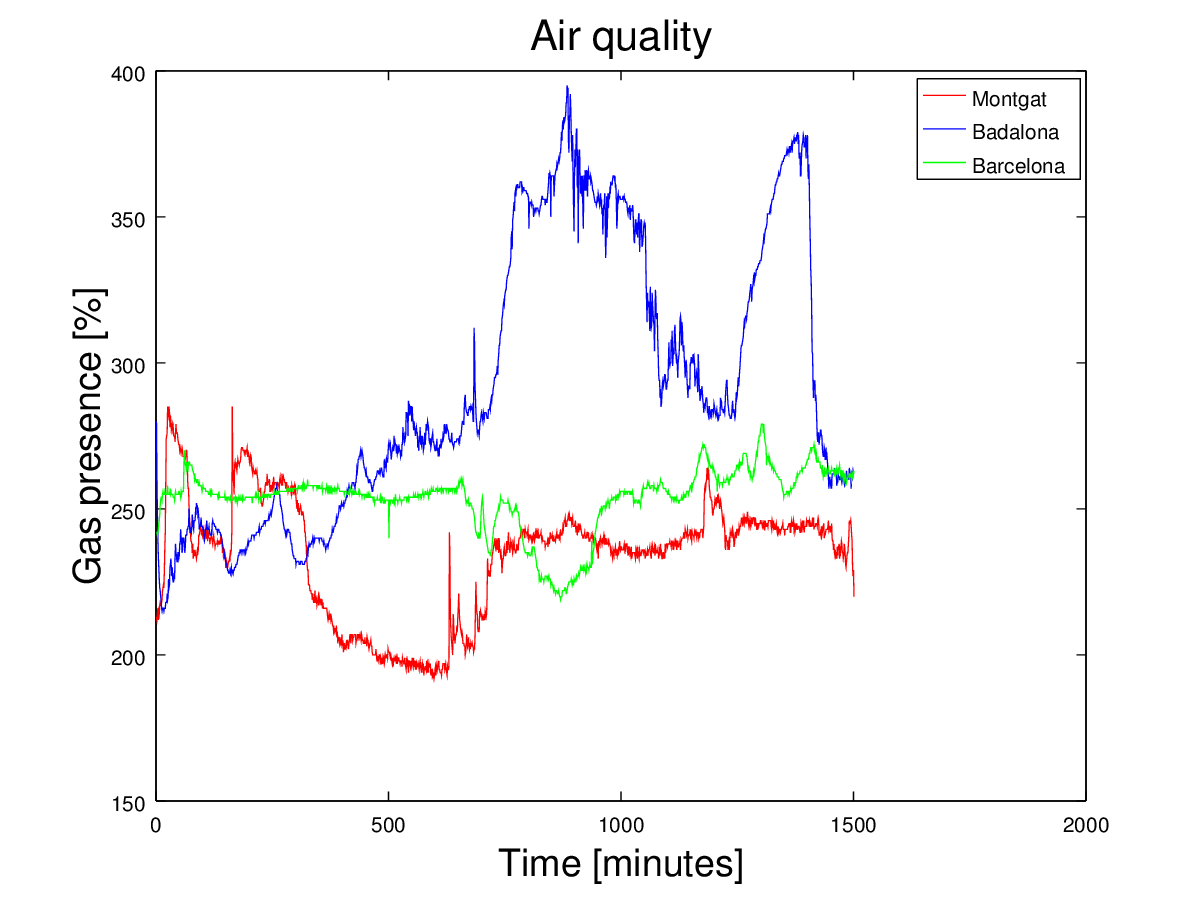
\includegraphics[page=1,scale=0.8]{./Figures/CompleteGraphicGas.png}
      \rule{35em}{0.5pt}
      \caption[Complete Graphic Air Quality]{Complete Graphic Air Quality.}
      \label{fig:CompleteGraphicGas}
    \end{figure}
    
    \begin{figure}[H]
      \centering
        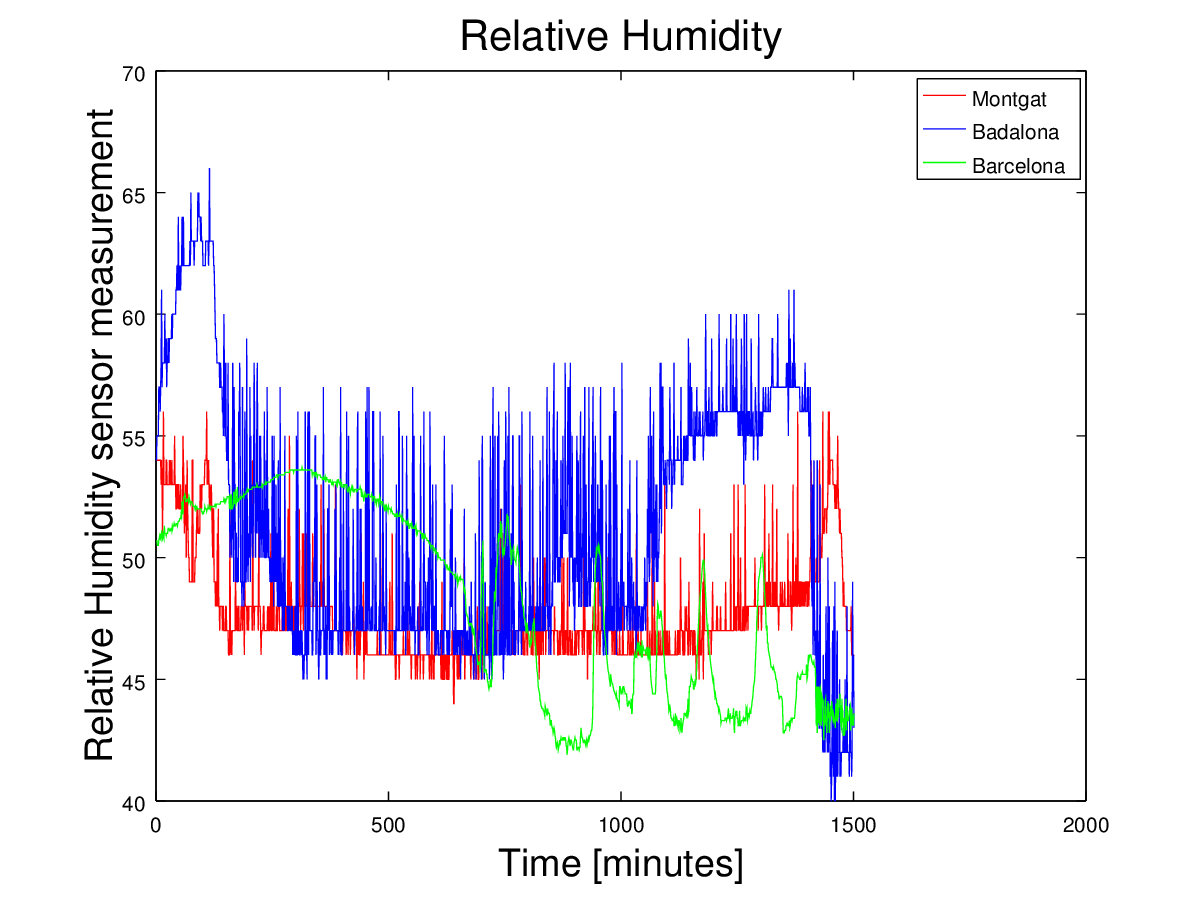
\includegraphics[page=1,scale=0.8]{./Figures/CompleteGraphicHumidity.png}
      \rule{35em}{0.5pt}
      \caption[Complete Graphic Humidity]{Complete Graphic Humidity.}
      \label{fig:CompleteGraphicHumidity}
    \end{figure}
    
    \begin{figure}[H]
      \centering
        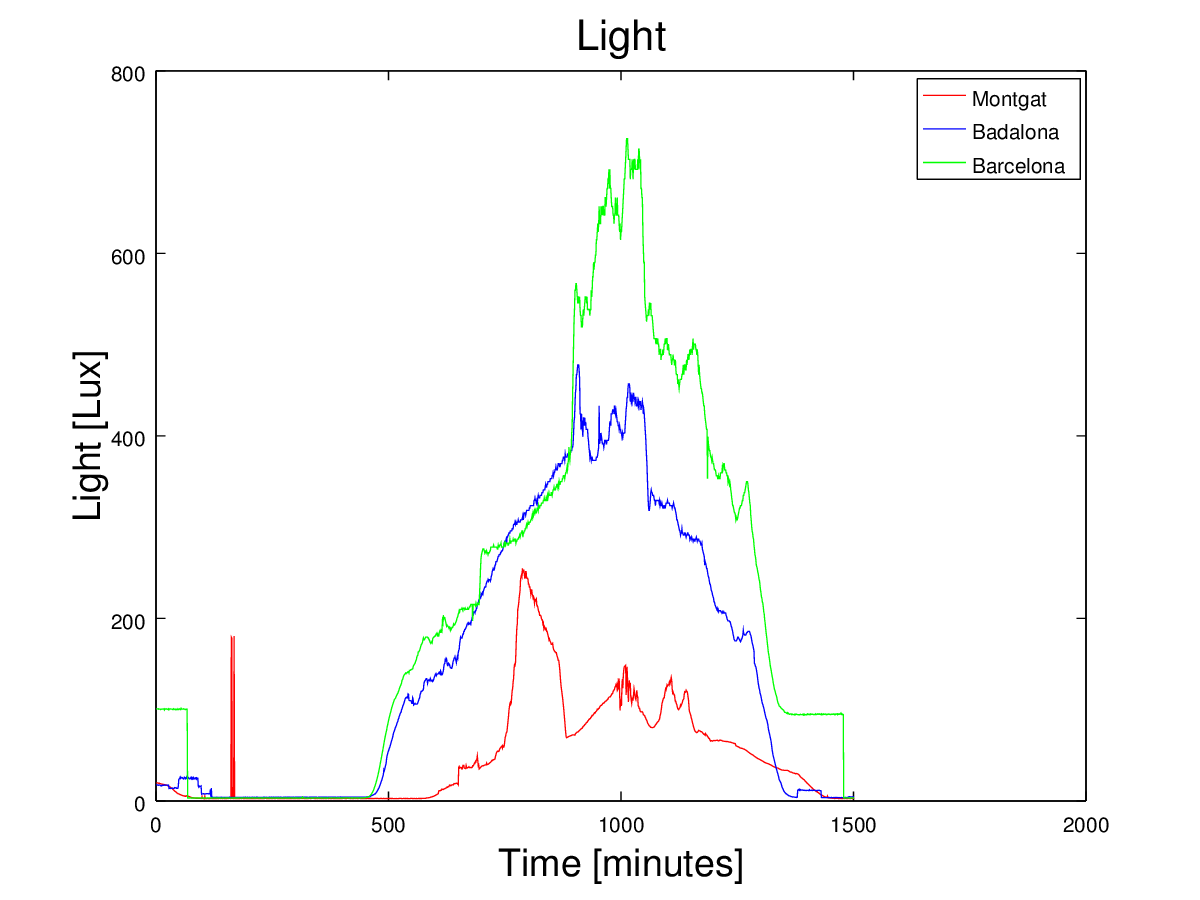
\includegraphics[page=1,scale=0.8]{./Figures/CompleteGraphicLight.png}
      \rule{35em}{0.5pt}
      \caption[Complete Graphic Light]{Complete Graphic Light.}
      \label{fig:CompleteGraphicLight}
    \end{figure}
    
    \begin{figure}[H]
      \centering
        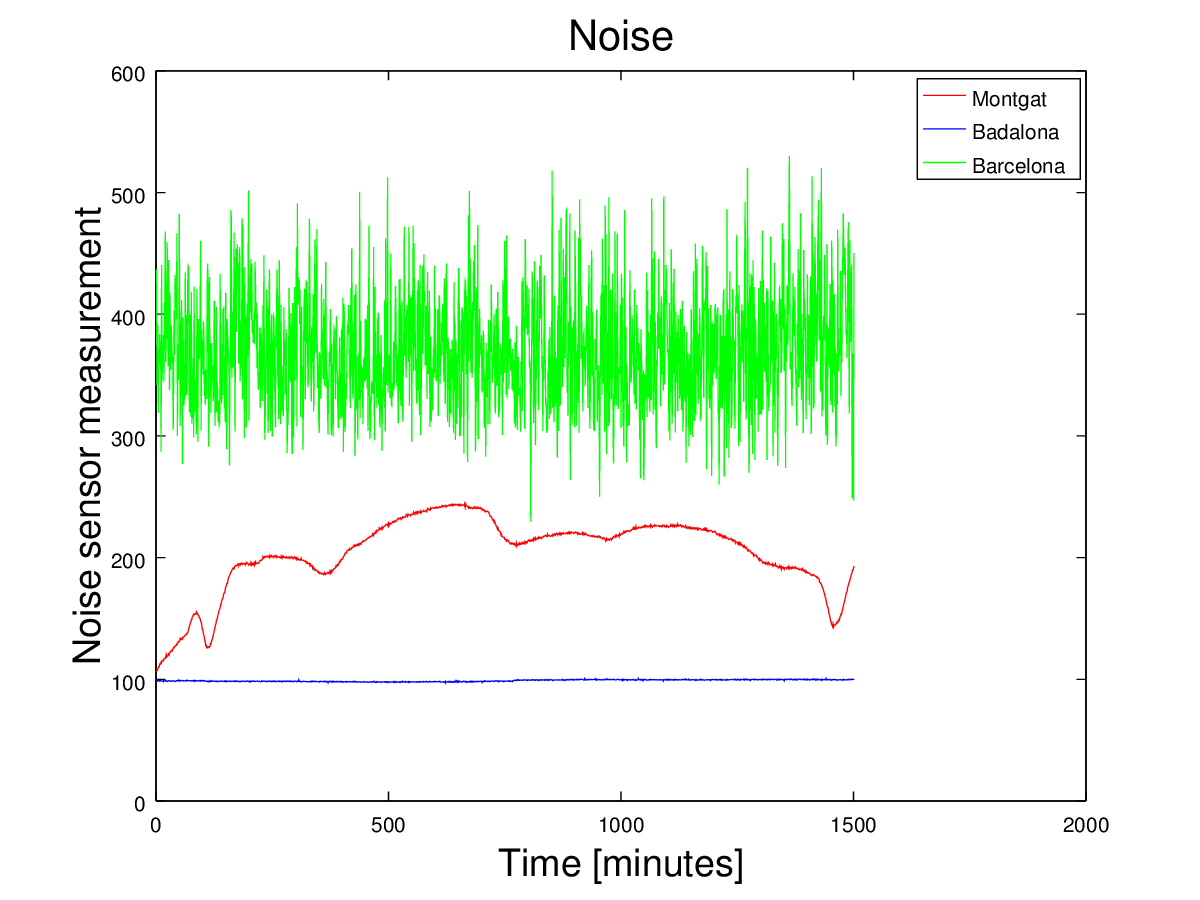
\includegraphics[page=1,scale=0.8]{./Figures/CompleteGraphicNoise.png}
      \rule{35em}{0.5pt}
      \caption[Complete Graphic Noise]{Complete Graphic Noise.}
      \label{fig:CompleteGraphicNoise}
    \end{figure}
    
    \begin{figure}[H]
      \centering
        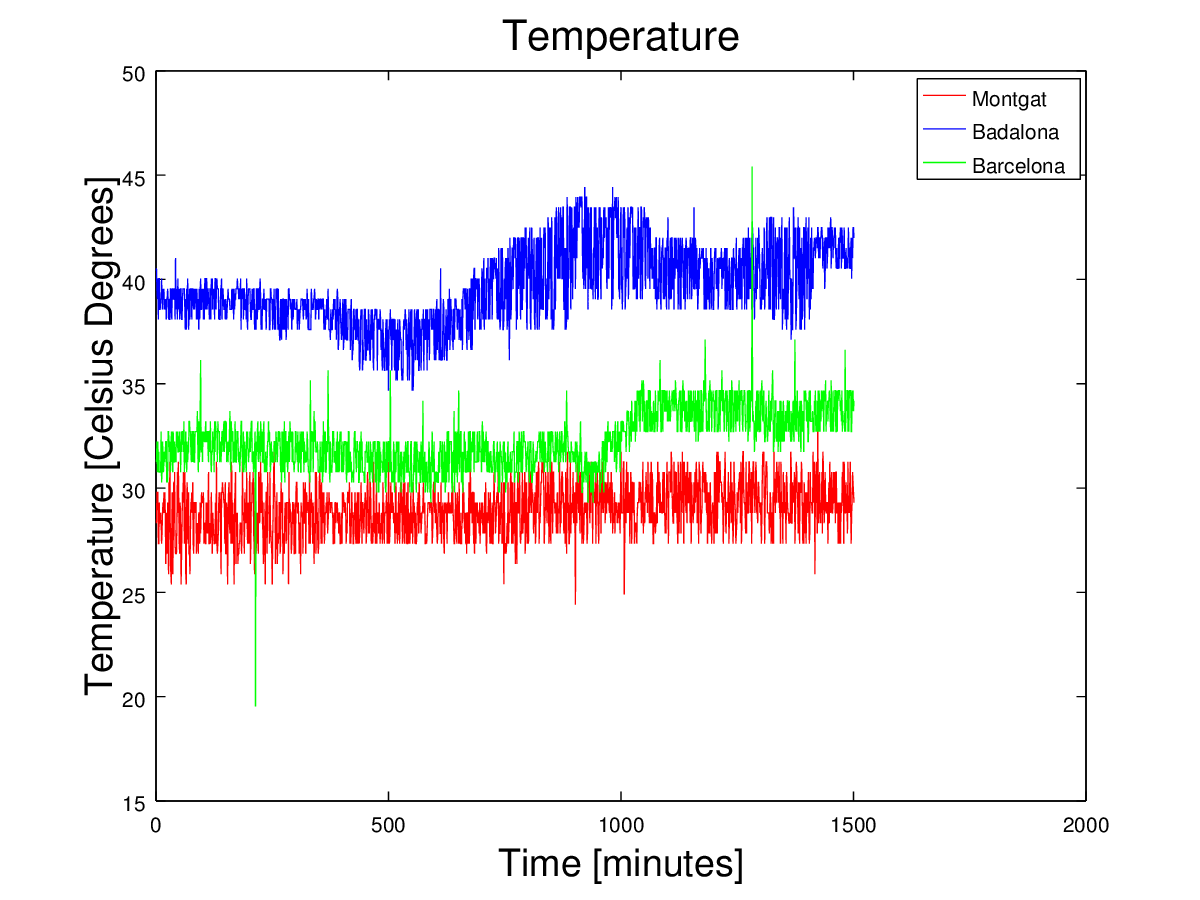
\includegraphics[page=1,scale=0.8]{./Figures/CompleteGraphicTemperature.png}
      \rule{35em}{0.5pt}
      \caption[Complete Graphic Temperature]{Complete Graphic Temperature.}
      \label{fig:CompleteGraphicTemperature}
    \end{figure}
  


\backmatter
\printindex





\end{document}


%NUMERACIÓ DE LA PÀGINA EXTERIOR EXCEPTE EN LA PRIMERA PÀGINA DE CADA CAPÍTOL
\usepackage{fancyhdr}
\pagestyle{fancy}
\fancyfoot{}
\fancyfoot[RO]{\thepage}
\fancyfoot[LE]{\thepage}


%MUTIPLES ÍNDEX
%En el preàmbul
\usepackage{multind}
\makeindex{authors}
%Introducció d'entrades la forma
\index{authors}{Einstein}
%Situació de l'Índex
\printindex{authors}{Author index}
%Cal eliminar les comandes \usepakage{makeidx} \makeindex \printindex
%cal exacutar des de la línia de comandes makeindex authors
